% Mid-evaluation slides, SDET Project 3. One file for the whole team.
% Build from inside this folder:  pdflatex main.tex   (run it twice)
% Figures come from ../figures/, so the slides always use the latest plots.
% Time limit: 20 to 25 minutes for the whole team, so each part has 5 to 8 frames.
% Each speaker writes in their own part below. Extra slides stay commented out.

\documentclass[aspectratio=169, 11pt]{beamer}
\usetheme{default}
\usecolortheme{default}
\setbeamertemplate{navigation symbols}{}
\setbeamertemplate{footline}[frame number]
\setbeamerfont{frametitle}{size=\large}
\setbeamercolor{frametitle}{fg=black}
\setbeamercolor{structure}{fg=blue!60!black}

\usepackage{amsmath, amssymb}
\usepackage{booktabs}
\usepackage{graphicx}
\graphicspath{{../figures/}}

\title{Loss Functions as Noise Models}
\subtitle{Signal Detection and Estimation Theory, Project 3}
\author{Varun Shastry \and Anshitha Penubolu \and Bhuvi \and Harsh}
\date{\today}

\begin{document}

\begin{frame}
  \titlepage
\end{frame}

% ============================================================
% PART 1 (Varun): report Sections 1 to 6, about 7 minutes
% ============================================================

\begin{frame}{The problem}
  \begin{itemize}
    \item Each loss function is the negative log-likelihood of one noise model.
    \item MSE assumes Gaussian noise. MAE assumes Laplace noise.
    \item \textbf{Question:} what is the cost when the noise model is wrong?
  \end{itemize}
  \vspace{0.6em}
  \textbf{Model.} We estimate a constant $A$ from $N$ samples:
  \[
    x[n] = A + w[n], \qquad n = 0, \dots, N-1, \qquad w[n] \text{ i.i.d., zero mean.}
  \]
  This is linear regression $\mathbf{y} = \mathbf{X}\boldsymbol\theta + \mathbf{w}$ with $\mathbf{X} = \mathbf{1}$.

  \vspace{0.6em}
  \textbf{Measure of cost.}
  \[
    \text{efficiency ratio} = \frac{\operatorname{Var}(\hat A)}{\text{CRLB}}
  \]
  A ratio of 2 means twice the variance of the best estimator. If both variances fall as 1/N, the estimator needs 2 times more data. If the variance stops falling, more data will not help.
\end{frame}

\begin{frame}{The loss comes from the noise model}
  \begin{columns}[T]
    \column{0.48\textwidth}
    \textbf{Gaussian noise}
    \[
      \ln p(\mathbf{x}; A) = c - \frac{1}{2\sigma^2}\sum_n (x[n] - A)^2
    \]
    The MLE minimises the squared error.
    \[
      \Rightarrow\ \hat A = \bar x \quad \text{(mean)}
    \]
    \column{0.48\textwidth}
    \textbf{Laplace noise}
    \[
      \ln p(\mathbf{x}; A) = c - \frac{1}{b}\sum_n |x[n] - A|
    \]
    The MLE minimises the absolute error.
    \[
      \Rightarrow\ \hat A = \operatorname{median}(\mathbf{x})
    \]
  \end{columns}
  \vspace{1em}
  \begin{itemize}
    \item For the median, the derivative of $\sum|x-A|$ is (samples below $A$) $-$ (samples above $A$). It changes sign at the middle sample.
    \item Choosing a loss is thus to choose a noise model!
  \end{itemize}
\end{frame}

\begin{frame}{CRLB and the predicted cost}
  \begin{columns}[T]
    \column{0.5\textwidth}
    \textbf{CRLB}
    \begin{itemize}
      \item Gaussian: $\sigma^2/N$
      \item Laplace: $b^2/N$
    \end{itemize}
    \textbf{Variance of each estimator}
    \begin{itemize}
      \item Mean: $\operatorname{Var}(w)/N$ (exact for all $N$)
      \item Median: $\approx 1/(4N\,p_w(0)^2)$ (large $N$)
    \end{itemize}
    \column{0.46\textwidth}
    \textbf{Predicted efficiency ratio}
    \vspace{0.4em}

    \begin{tabular}{lcc}
      \toprule
       & Gaussian & Laplace \\
      \midrule
      Mean (MSE)   & $1$     & $2$ \\
      Median (MAE) & $\pi/2$ & $1$ \\
      \bottomrule
    \end{tabular}
  \end{columns}
  \vspace{1.2em}
  \begin{itemize}
    \item Each estimator is best only for its own noise.
    \item Under Laplace noise, the mean needs 2 times more data than the median.
  \end{itemize}
\end{frame}

\begin{frame}{Simulation with Gaussian and Laplace noise}
  \begin{columns}[c]
    \column{0.58\textwidth}
    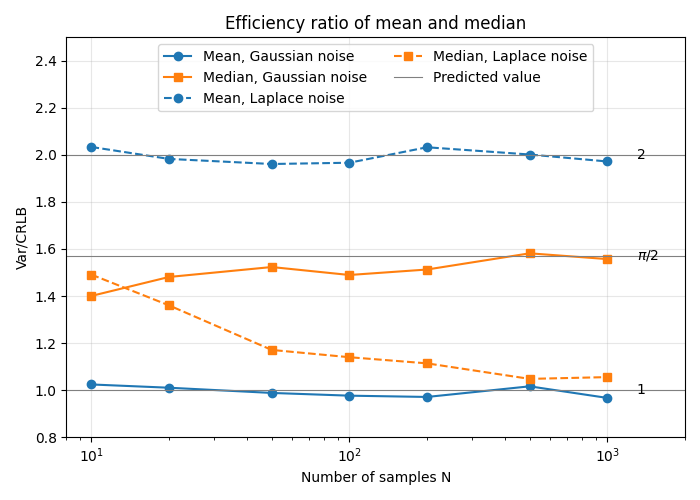
\includegraphics[width=\linewidth]{simA_ratio_vs_N.png}
    \column{0.40\textwidth}
    \small
    $5000$ trials. Measured at $N = 100$:

    \vspace{0.4em}
    \begin{tabular}{lcc}
      \toprule
       & Gauss. & Laplace \\
      \midrule
      Mean   & 0.97 & 2.01 \\
      Median & 1.51 & 1.17 \\
      \bottomrule
    \end{tabular}

    \vspace{0.8em}
    \begin{itemize}
      \item The mean is flat for all $N$.
      \item The median reaches its value only for large $N$.
      \item At small N, our median results match exact published values (NIST, 1964).
    \end{itemize}
  \end{columns}
\end{frame}

\begin{frame}{Skewed noise: the loss changes the target}
  \begin{columns}[c]
    \column{0.68\textwidth}
    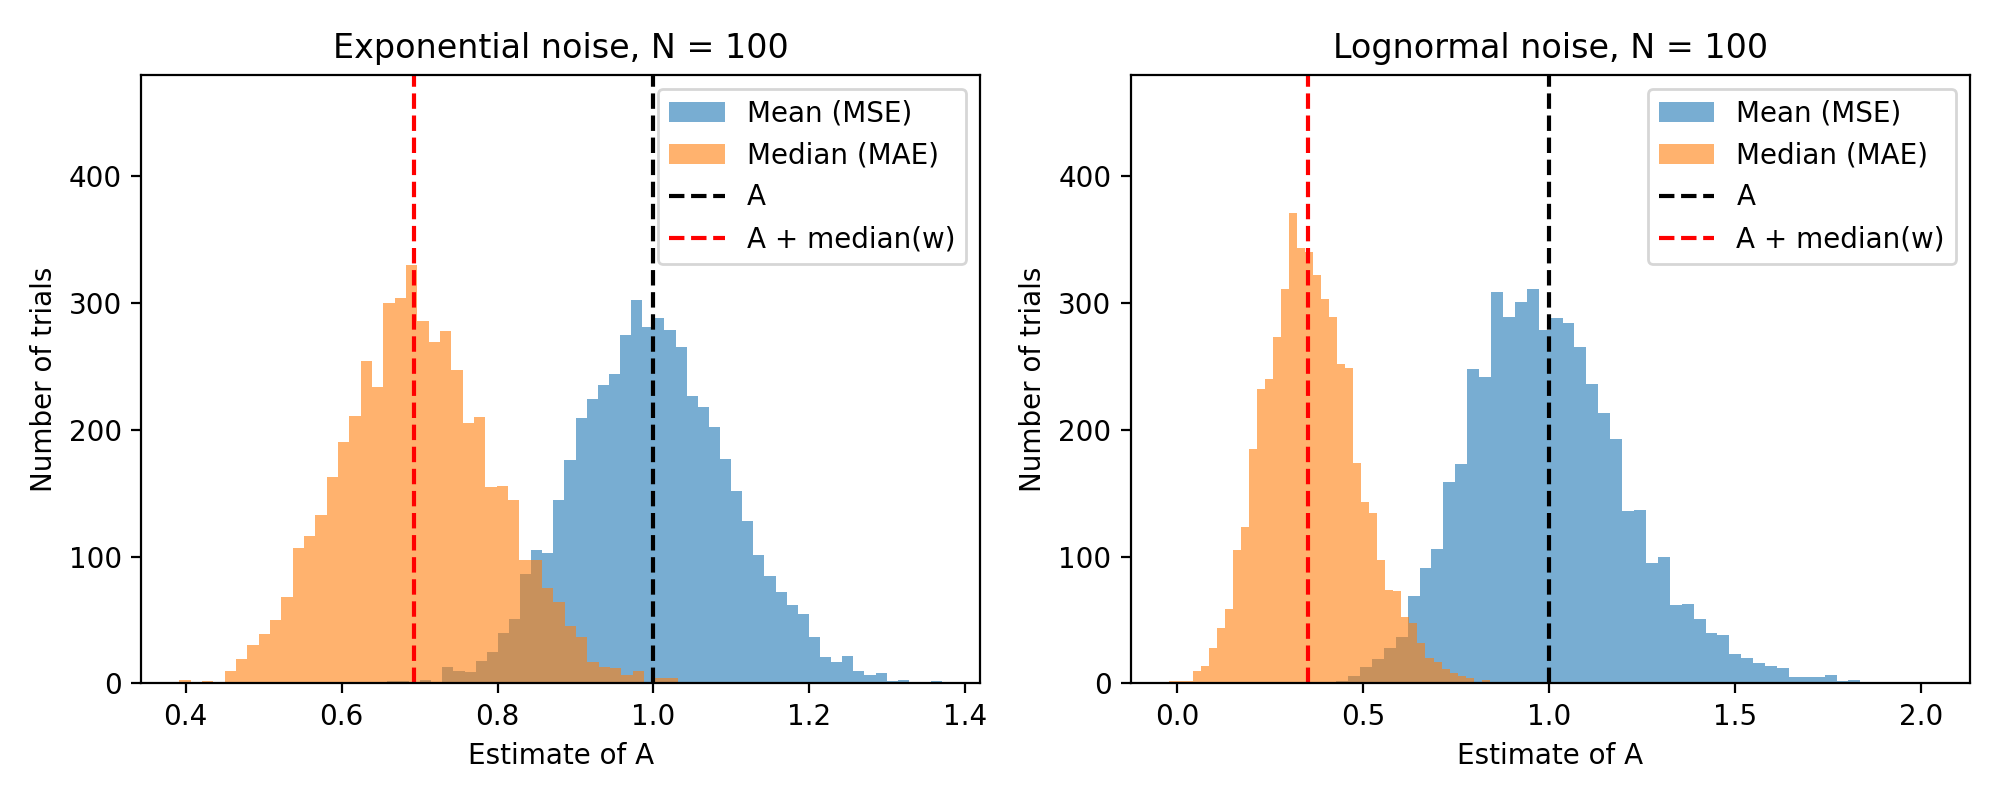
\includegraphics[width=\linewidth]{simB_histograms.png}
    \column{0.31\textwidth}
    \small
    Consider the case of zero-mean noise, but now not symmetric!
    \begin{itemize}
      \item Mean = $A$
      \item Median = $A + \operatorname{median}(w)$
    \end{itemize}
    \vspace{0.3em}
    \begin{tabular}{@{}lcc@{}}
      \toprule
       & Pred. & Meas. \\
      \midrule
      Expon. & 0.693 & 0.698 \\
      Lognorm. & 0.351 & 0.363 \\
      \bottomrule
    \end{tabular}

    \vspace{0.5em}
    MSE is not biased. MSE and MAE estimate different values.
  \end{columns}
\end{frame}

\begin{frame}{Student-t noise: the model}
  \[
    p_w(w) = \frac{\Gamma\!\left(\frac{\nu+1}{2}\right)}{\sqrt{\nu\pi}\,\Gamma\!\left(\frac{\nu}{2}\right)s}
    \left(1 + \frac{w^2}{\nu s^2}\right)^{-\frac{\nu+1}{2}}
  \]
  \vspace{-0.6em}
  \begin{center}
    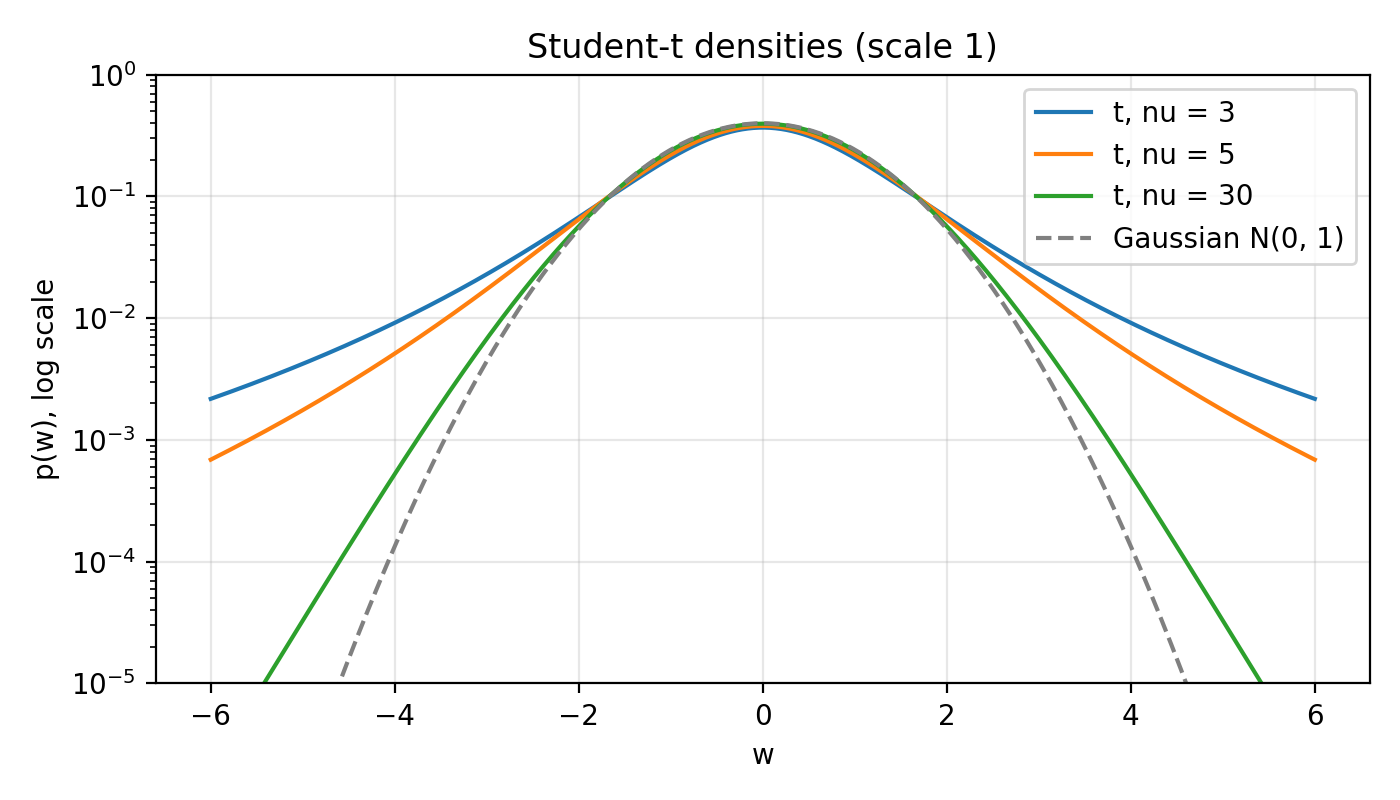
\includegraphics[width=0.95\linewidth]{simC_t_density.png}
  \end{center}
  \vspace{-0.6em}
  \small
  \begin{itemize}
    \item $\nu$ sets the tails. $\nu \to \infty$ gives Gaussian. $\nu = 1$ gives Cauchy.
    \item $s$ sets the width. $\operatorname{Var}(w) = s^2\nu/(\nu - 2)$, finite only for $\nu > 2$.
    \item It is a Gaussian with a random variance (Lange et al., 1989).
  \end{itemize}
\end{frame}

\begin{frame}{Student-t noise: results}
  \begin{columns}[c]
    \column{0.52\textwidth}
    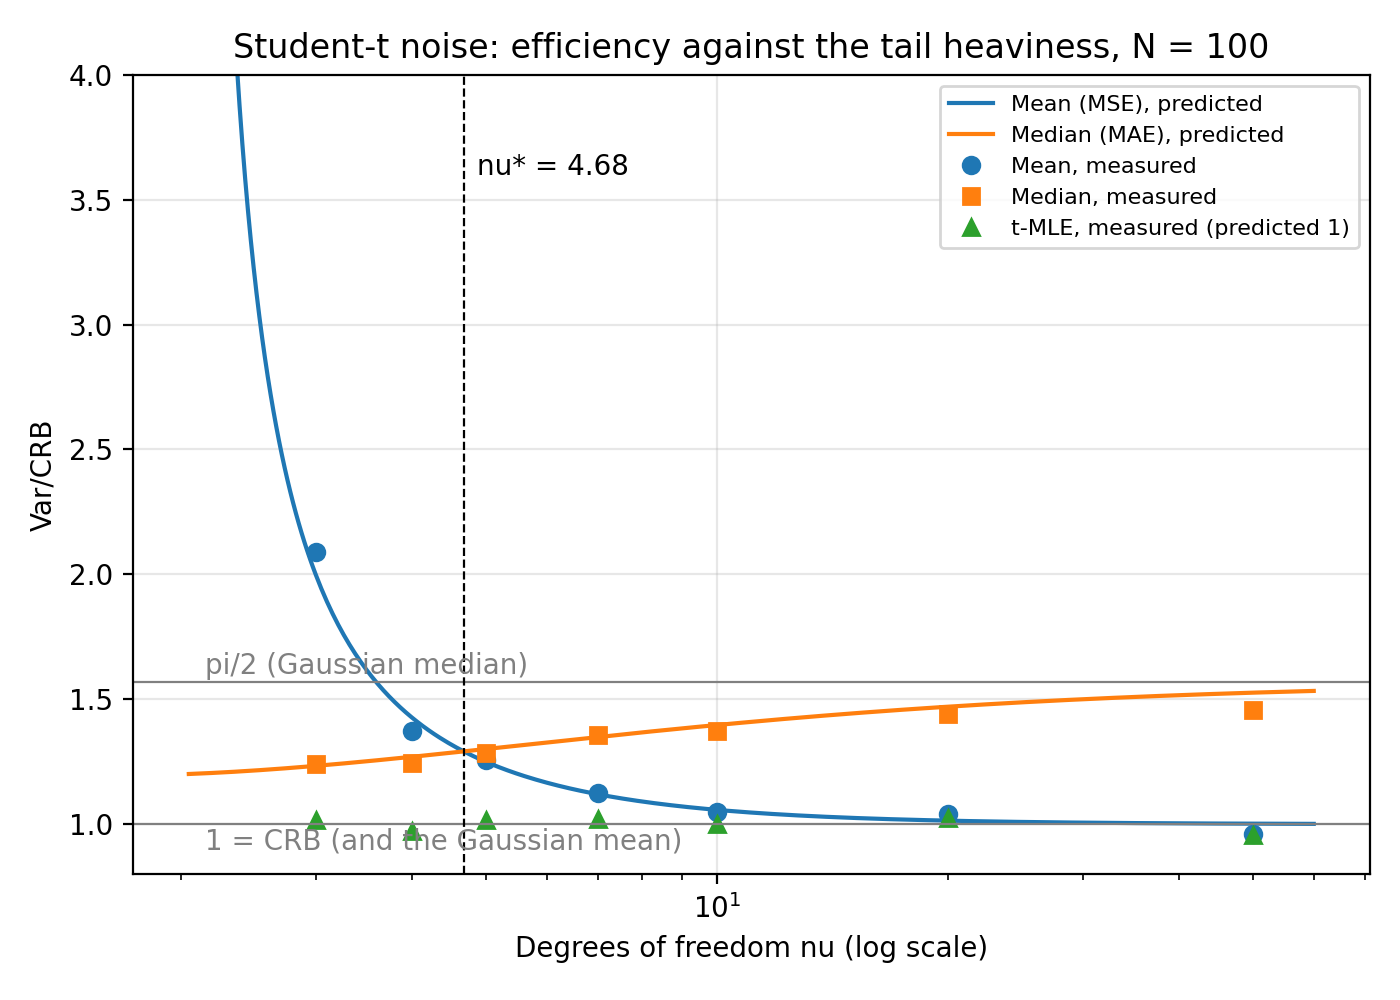
\includegraphics[width=\linewidth]{simC_ratio_vs_nu.png}
    \column{0.46\textwidth}
    \small
    \[
      \text{CRLB} = \frac{\nu+3}{\nu+1}\cdot\frac{s^2}{N}
    \]
    \[
      \frac{\operatorname{Var}(\bar x)}{\text{CRLB}} = \frac{\nu(\nu+1)}{(\nu-2)(\nu+3)}
    \]
    \begin{itemize}
      \item Heavy tails make the mean much worse (leftwards in the plot).
      \item The median stays between 1.2 and 1.5.
      \item They are equal at $\nu \approx 4.68$.
      \item The t-MLE is a weighted mean with weight $(\nu+1)/(\nu + r^2)$. It reaches the CRLB.
    \end{itemize}
  \end{columns}
\end{frame}

% \begin{frame}{Summary of part 1}
%   \begin{itemize}
%     \item Each loss is optimal only for its own noise model.
%     \item Symmetric noise: the wrong loss costs variance ($2\times$ or $\pi/2\times$).
%     \item Skewed noise: the wrong loss changes the value that it estimates.
%     \item Heavy tails: MSE gets worse quickly. MAE stays within about 1.5 times the CRLB. The matched loss reaches the CRLB.
%     \item All predictions agree with simulation.
%   \end{itemize}
% \end{frame}


% ============================================================
% BACKUP SLIDES for part 1. Remove the % signs to use them.
% ============================================================

% \appendix
%
% \begin{frame}{Backup: CRLB for Laplace noise}
%   \begin{itemize}
%     \item Score of one sample: $\dfrac{\partial}{\partial A}\ln p = \dfrac{\operatorname{sign}(x - A)}{b}$, so its square is $1/b^2$.
%     \item Fisher information $N/b^2$, so $\text{CRLB} = b^2/N$.
%     \item We use $I = E[(\partial \ln p/\partial A)^2]$. The form $-E[\partial^2 \ln p/\partial A^2]$ gives $0$, because $\ln p$ has a corner at $x = A$.
%     \item The corner has probability zero, so the bound is valid.
%   \end{itemize}
% \end{frame}
%
% \begin{frame}{Backup: Student-t with infinite variance ($\nu \le 2$)}
%   \begin{columns}[c]
%     \column{0.62\textwidth}
%     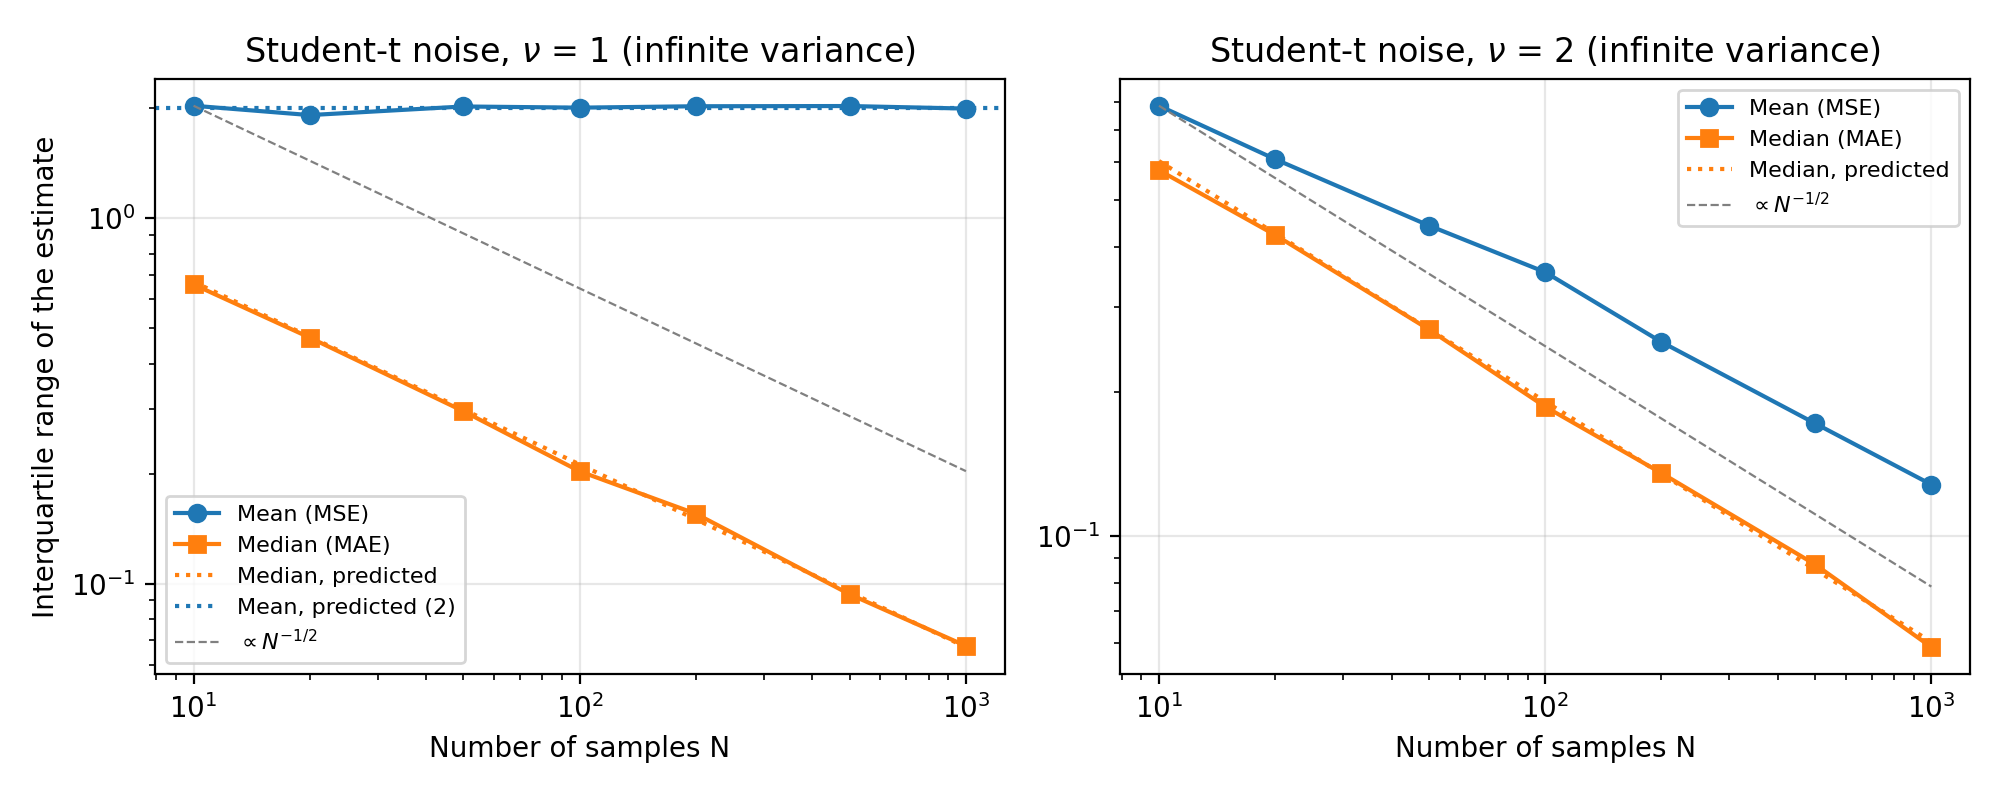
\includegraphics[width=\linewidth]{simC_infinite_variance.png}
%     \column{0.36\textwidth}
%     \small
%     We compare the interquartile range (IQR), because the variance is infinite.
%     \begin{itemize}
%       \item $\nu = 1$ (Cauchy): the mean of $N$ samples has the same distribution as one sample. Its IQR stays at 2.
%       \item The median IQR decreases as $1/\sqrt{N}$.
%     \end{itemize}
%   \end{columns}
% \end{frame}
%
% \begin{frame}{Backup: Student-t, ratio against $N$}
%   \begin{center}
%     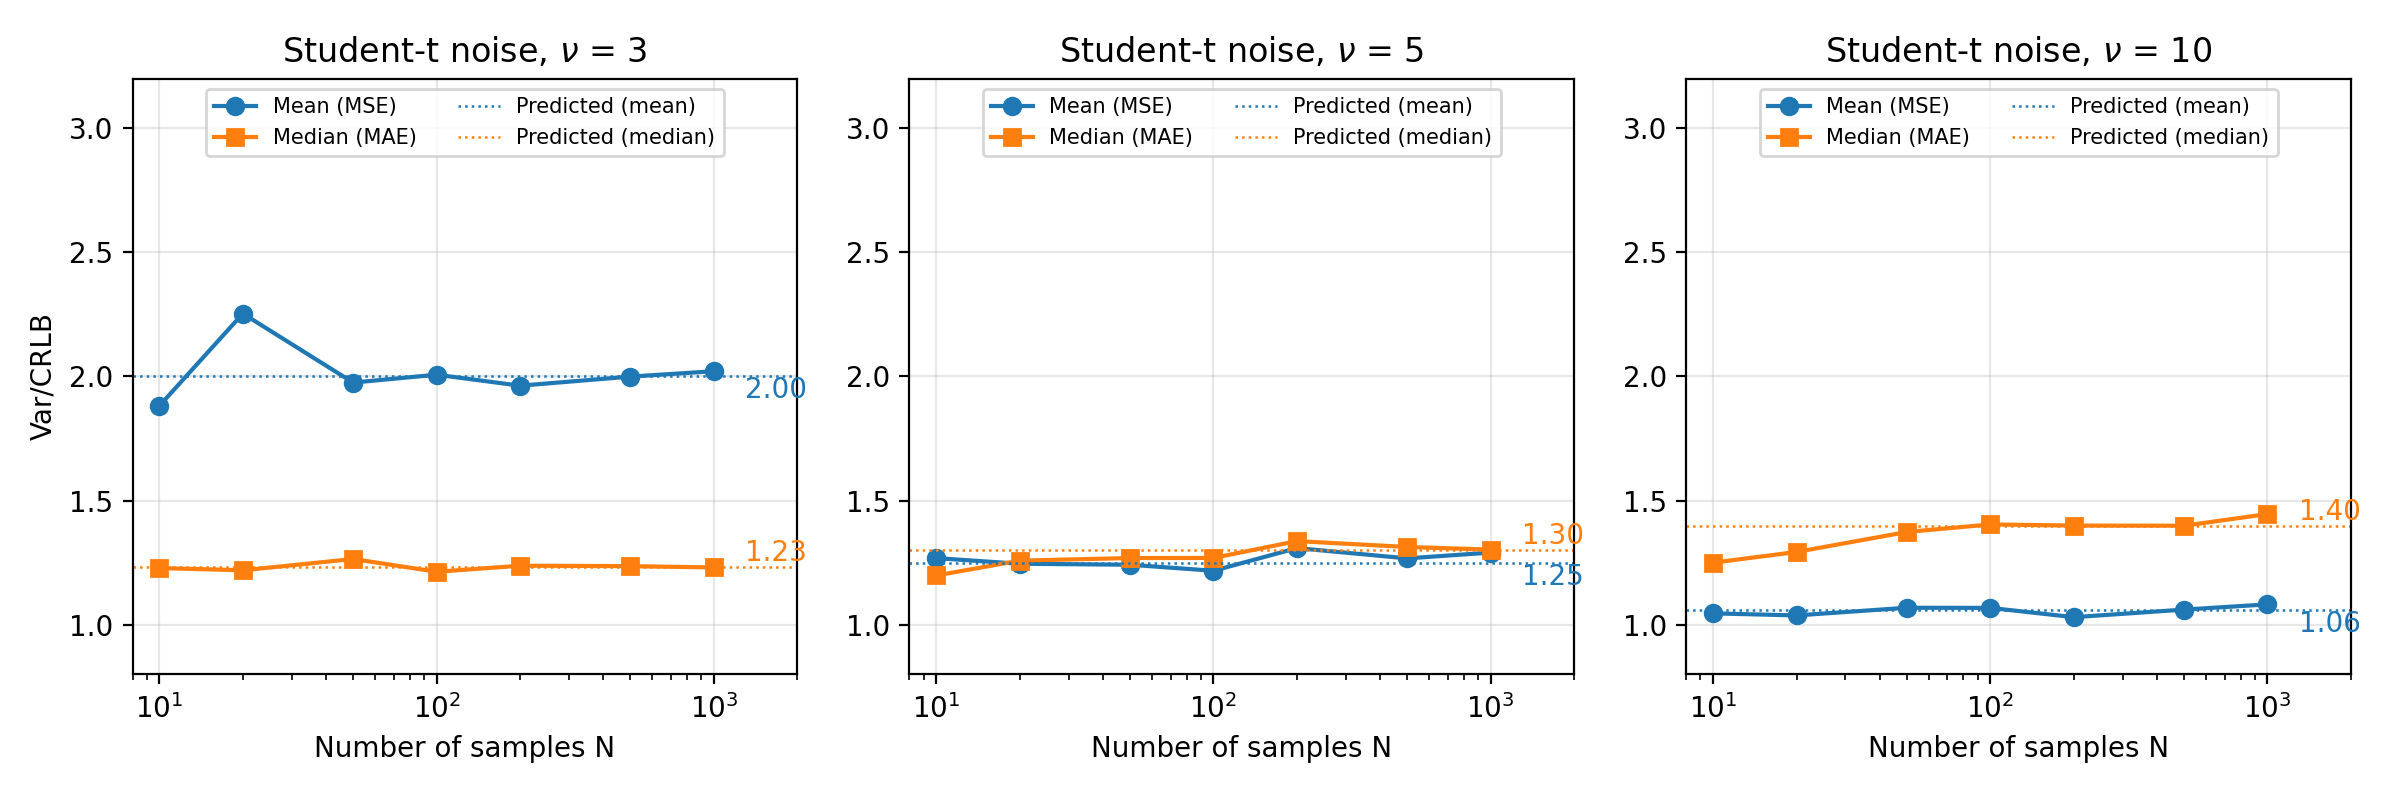
\includegraphics[width=\linewidth]{simC_ratio_vs_N.png}
%   \end{center}
%   \small The mean is flat for all $N$. The median settles after a few hundred samples.
% \end{frame}


% PART 2 (Bhuvi): the misspecified CRB, report Section 8, about 8 minutes
% ============================================================

\begin{frame}{Why we need a new bound}
  \begin{itemize}
    \item The CRLB is computed from the \textbf{true} noise. An estimator built on the \textbf{wrong} noise model never reaches it.
    \item The mean under Laplace noise stays at $2\times$ CRLB for every $N$. The median under skewed noise does not even aim at $A$.
    \item We want a bound that predicts what the wrong-model estimator \textbf{actually} gets.
  \end{itemize}
  \vspace{0.5em}
  \textbf{Example.} Estimate the noise variance with a Gaussian model, $\hat\theta = \frac1N\sum_n x[n]^2$, when the noise is Laplace($b$):
  \vspace{0.3em}
  \begin{center}
    \begin{tabular}{lc}
      \toprule
      Bound & $N \cdot$ value \\
      \midrule
      CRLB of the assumed Gaussian model & $8b^4$ \\
      CRLB of the true Laplace model & $16b^4$ \\
      Actual variance of $\hat\theta$ (measured $20.04$) & $\mathbf{20b^4}$ \\
      \bottomrule
    \end{tabular}
  \end{center}
  \vspace{0.3em}
  Trusting the wrong model gives $8b^4$, which is not even a valid bound. The true CRLB is valid, but loose.
\end{frame}

\begin{frame}{The misspecified CRB (MCRB)}
  True density $p$, assumed model $f(x \mid \theta)$.
  \begin{columns}[T]
    \column{0.52\textwidth}
    \textbf{Pseudo-true parameter} (closest model in KL)
    \[
      \theta_0 = \arg\max_\theta\, E_p\big[\ln f(x\mid\theta)\big]
    \]
    \textbf{MCRB} (Vuong 1986, Fortunati et al.\ 2017)
    \[
      \text{MCRB} = \frac{1}{N}\,\frac{\mathcal B}{\mathcal A^2}, \quad
      \begin{aligned}
        \mathcal A &= E_p[\partial_\theta^2 \ln f]\\
        \mathcal B &= E_p[(\partial_\theta \ln f)^2]
      \end{aligned}
    \]
    Model inside, true density outside.
    \column{0.46\textwidth}
    \textbf{Two key facts}
    \begin{itemize}
      \item Correct model: $\mathcal B = -\mathcal A = I$, so MCRB = CRLB.
      \item The wrong-model MLE goes to $\theta_0$ with variance $\to$ MCRB. So the bound is \textbf{tight}.
    \end{itemize}
    \textbf{Our earlier formulas are MCRBs}
    \begin{itemize}
      \item Gaussian model: mean, $\operatorname{Var}(w)/N$
      \item Laplace model: median, $1/(4N f(m)^2)$, aiming at $A + \operatorname{median}(w)$
    \end{itemize}
  \end{columns}
  \vspace{0.4em}
  \centering Efficiency ratio $=$ MCRB / CRLB $=$ the price of the wrong model.
\end{frame}

\begin{frame}{Which estimators does the MCRB bound?}
  \textbf{Paradox.} Laplace noise, Gaussian model: MCRB $= 2b^2/N$. The median is unbiased for $\theta_0 = A$, yet has variance $b^2/N$.

  \vspace{0.5em}
  \textbf{Resolution.} The bound needs $E_p[\hat\theta] = \theta_0(p)$ for \textbf{every} true $p$, not only ours.
  \begin{itemize}
    \item Perturb the truth: $p_t = p\,(1 + t\,g)$. Unbiasedness along $p_t$ plus Cauchy--Schwarz gives
    \[
      \operatorname{Var}(\hat\theta) \geq \frac{(E[\phi\, g])^2}{N\,E[g^2]}, \qquad \phi = -\frac{\partial_\theta \ln f}{\mathcal A}.
    \]
    \item The best direction is $g = \phi$, which gives exactly $\mathcal B/(N\mathcal A^2)$.
    \item Along that direction, $\theta_0$ moves at rate $2b^2$ but the median moves at $b^2$. So the median is \textbf{not covered}.
  \end{itemize}
  \vspace{0.3em}
  \textbf{So:} one loss's MCRB is not a floor for other losses. The common floor is the CRLB of the true noise.
\end{frame}

\begin{frame}{Regression with robust losses: one formula}
  $y_i = \theta_0 + \theta_1 x_i + w_i$, \quad $x_i \sim U(-2,2)$, \quad loss $\rho$ with $\psi = \rho'$.
  \begin{columns}[T]
    \column{0.52\textwidth}
    \textbf{Linearise} $\sum_i \psi(y_i - \mathbf x_i^\top\hat{\boldsymbol\theta})\,\mathbf x_i = \mathbf 0$:
    \[
      \text{MCRB} = \frac{\kappa}{\lambda^2}\,(\mathbf X^\top\mathbf X)^{-1}, \qquad
      \text{CRLB} = \frac{(\mathbf X^\top\mathbf X)^{-1}}{I_{\text{loc}}}
    \]
    $\lambda = E[\psi'(w)]$, \ $\kappa = E[\psi(w)^2]$ (MAE: $\lambda = 2p(0)$).
    \[
      \text{ratio} = \frac{\kappa\, I_{\text{loc}}}{\lambda^2} \;\geq\; 1
    \]
    By Cauchy--Schwarz, with $=1$ only for the true likelihood.
    \column{0.45\textwidth}
    \small
    \textbf{Losses:} MSE, MAE, Huber, $t_3$, Cauchy.\\
    \textbf{Noises:} Gaussian, Laplace, $t_3$, Cauchy, contaminated $0.9\,\mathcal N(0,1) + 0.1\,\mathcal N(0,25)$.
    \vspace{0.4em}
    \begin{itemize}
      \item Symmetric noise: every loss aims at the true $\boldsymbol\theta$.
      \item Scale rule fixed beforehand: each loss uses the scale that makes it the MLE for its own noise, estimated from the MAD.
      \item The ratio does not depend on $\mathbf X$.
    \end{itemize}
  \end{columns}
\end{frame}

\begin{frame}{Mismatch matrix: predicted vs measured}
  \begin{columns}[c]
    \column{0.62\textwidth}
    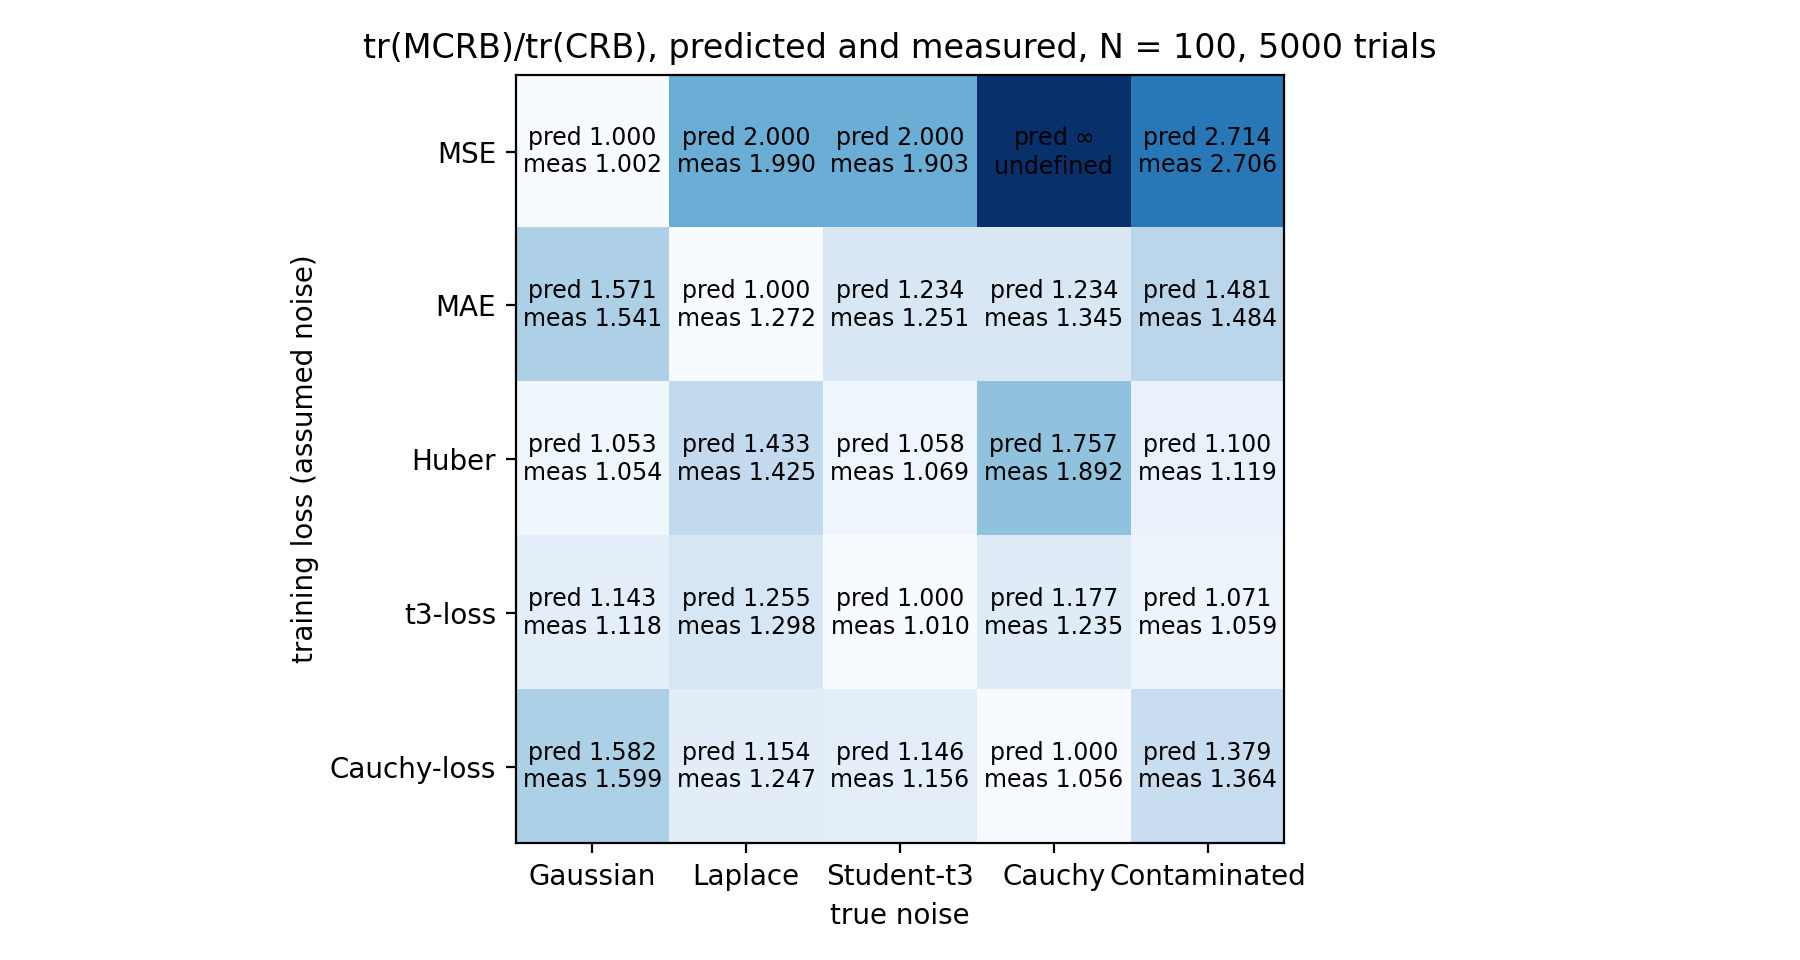
\includegraphics[width=\linewidth, trim=90 0 120 0, clip]{simJ_mismatch_matrix.png}
    \column{0.37\textwidth}
    \small
    $N = 100$, $5000$ trials per cell.
    \begin{itemize}
      \item Diagonal $= 1$. No loss is best everywhere.
      \item MSE fails under Cauchy noise: $\kappa = E[w^2] = \infty$.
      \item Gates: MSE $\approx 1, 2$ under Gaussian and Laplace, $t_3$-loss at $1.01$.
      \item 16 of 24 cells within 2 standard errors. All biases $< 0.005$.
      \item The rest are above the prediction: finite-$N$ effects. At $N = 1000$ they are within $4\%$.
    \end{itemize}
  \end{columns}
\end{frame}

\begin{frame}{How tight is the MCRB at finite $N$?}
  \begin{columns}[c]
    \column{0.6\textwidth}
    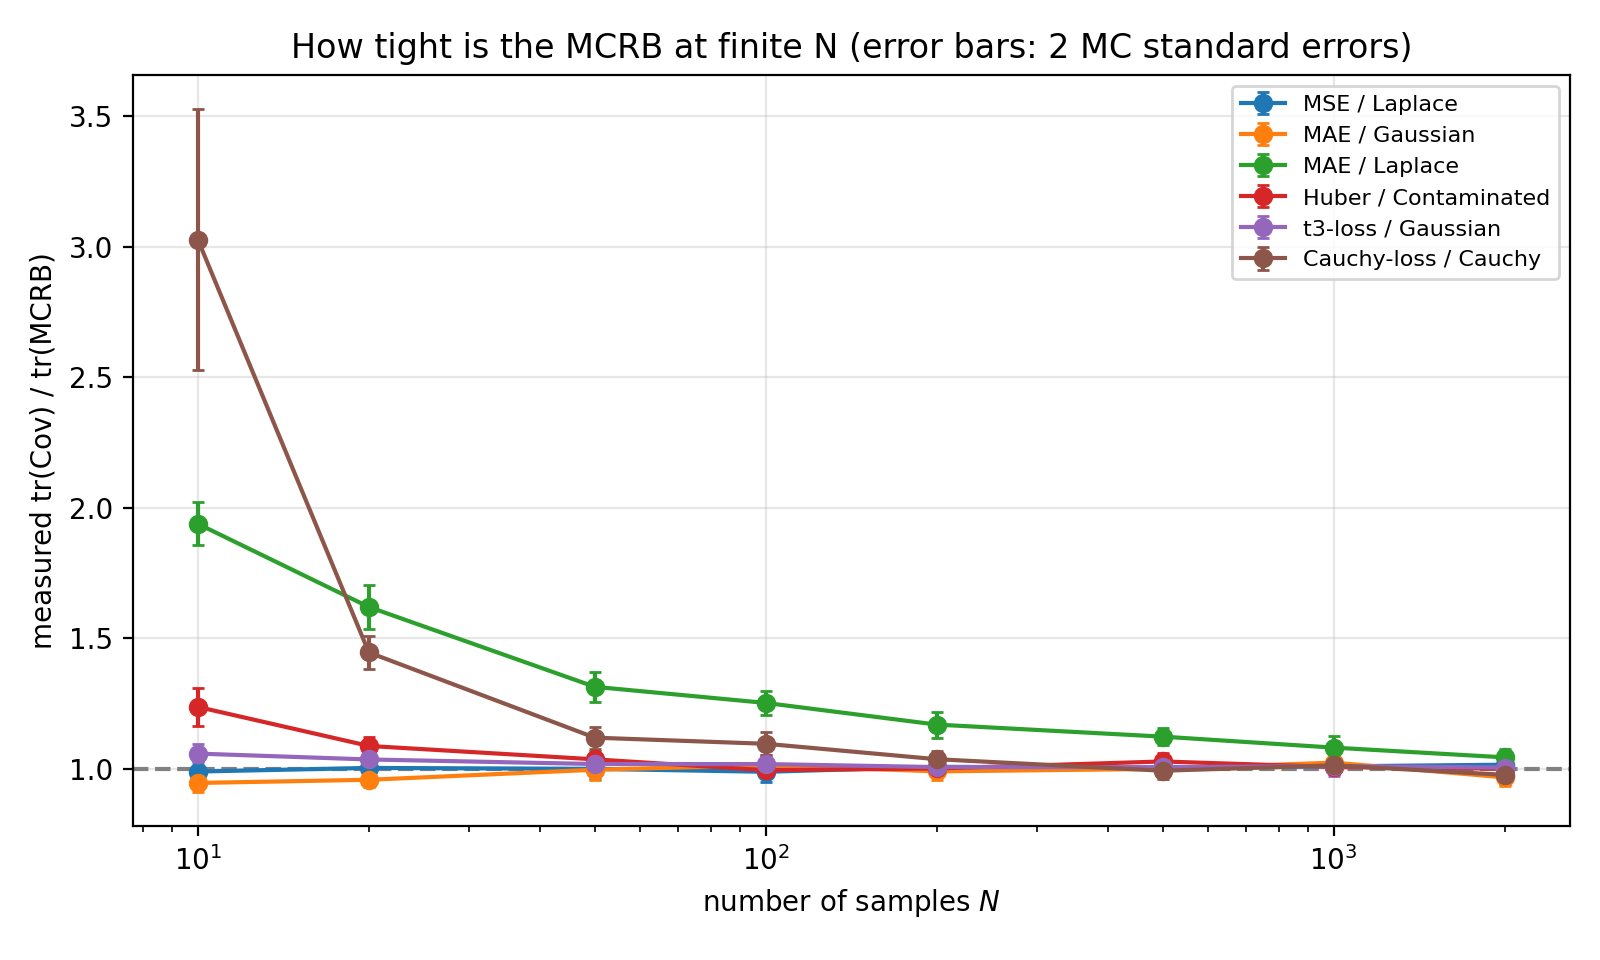
\includegraphics[width=\linewidth]{simJ_tightness_vs_N.png}
    \column{0.39\textwidth}
    \small
    Measured variance $/$ MCRB, $4000$ trials.
    \begin{itemize}
      \item \textbf{Exact for all $N$:} MSE (OLS is linear in the data).
      \item \textbf{Slowly from above:} MAE under Laplace, $1.94 \to 1.04$. Cauchy-loss, $3.0$ at $N = 10$.
      \item \textbf{Below the bound:} MAE under Gaussian, $0.942 \pm 0.006$ at $N = 10$.
    \end{itemize}
    \vspace{0.3em}
    The MCRB is reached in the limit. It is not a finite-$N$ floor.
  \end{columns}
\end{frame}

\begin{frame}{Estimating the MCRB from data (sandwich)}
  \begin{center}
    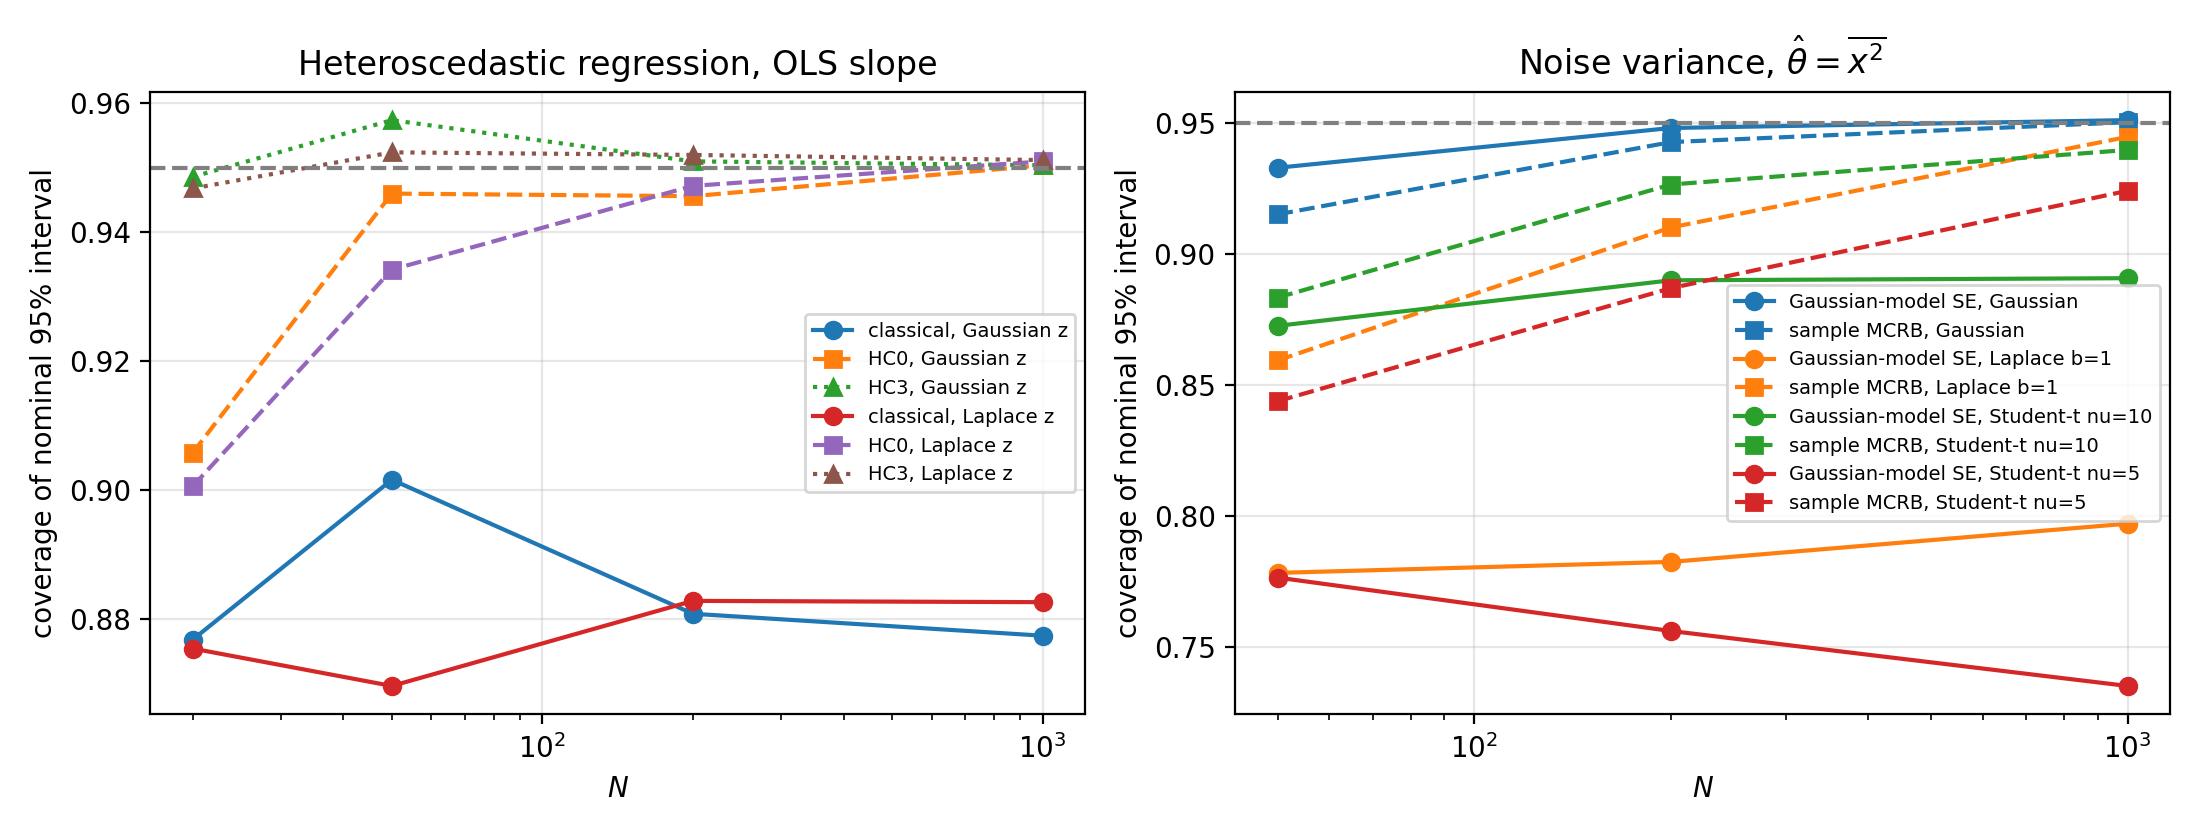
\includegraphics[width=0.82\linewidth]{simK_sandwich_coverage.png}
  \end{center}
  \vspace{-0.4em}
  \small
  $\widehat{\text{Cov}} = \hat{\mathbf A}^{-1}\hat{\mathbf B}\hat{\mathbf A}^{-1}$ from the residuals. Coverage of $95\%$ intervals, $5000$ trials:
  \begin{itemize}
    \item \textbf{Heteroscedastic regression:} classical SE about $88\%$ at every $N$. HC3 (sandwich) about $95\%$ from $N = 20$.
    \item \textbf{Noise variance, Laplace:} Gaussian-model SE $78$--$80\%$ (predicted $78.5\%$). Sandwich reaches $94.5\%$ at $N = 1000$.
  \end{itemize}
\end{frame}

\begin{frame}{Summary of part 2}
  \begin{itemize}
    \item The CRLB says what is possible. The MCRB says what the wrong model actually gets.
    \item MCRB / CRLB is the price of the wrong loss, and one formula $\kappa\lambda^{-2}(\mathbf X^\top\mathbf X)^{-1}$ predicts all 25 cells.
    \item It binds only estimators unbiased for $\theta_0(p)$ for every $p$. Compare losses against the true CRLB.
    \item Tight as $N \to \infty$. At small $N$ it can be above or below.
    \item From data, the sandwich gives correct intervals where the model-based formula does not.
  \end{itemize}
\end{frame}

% ============================================================
% BACKUP SLIDES for part 2. Remove the % signs to use them.
% ============================================================

% \begin{frame}{Backup: predicted mismatch matrix, $\kappa I_{\text{loc}}/\lambda^2$}
%   \centering
%   \begin{tabular}{lccccc}
%     \toprule
%     Loss & Gaussian & Laplace & $t_3$ & Cauchy & Contam. \\
%     \midrule
%     MSE         & 1     & 2     & 2     & $\infty$ & 2.714 \\
%     MAE         & 1.571 & 1     & 1.234 & 1.234 & 1.481 \\
%     Huber       & 1.053 & 1.433 & 1.058 & 1.757 & 1.100 \\
%     $t_3$-loss  & 1.143 & 1.255 & 1     & 1.177 & 1.071 \\
%     Cauchy-loss & 1.582 & 1.154 & 1.146 & 1     & 1.379 \\
%     \bottomrule
%   \end{tabular}
% \end{frame}

% ---------- Anshitha: gamma noise (report Section 7), about 2 minutes ----------

\begin{frame}{Skewed noise: the gamma family}
  \begin{columns}[c]
    \column{0.55\textwidth}
    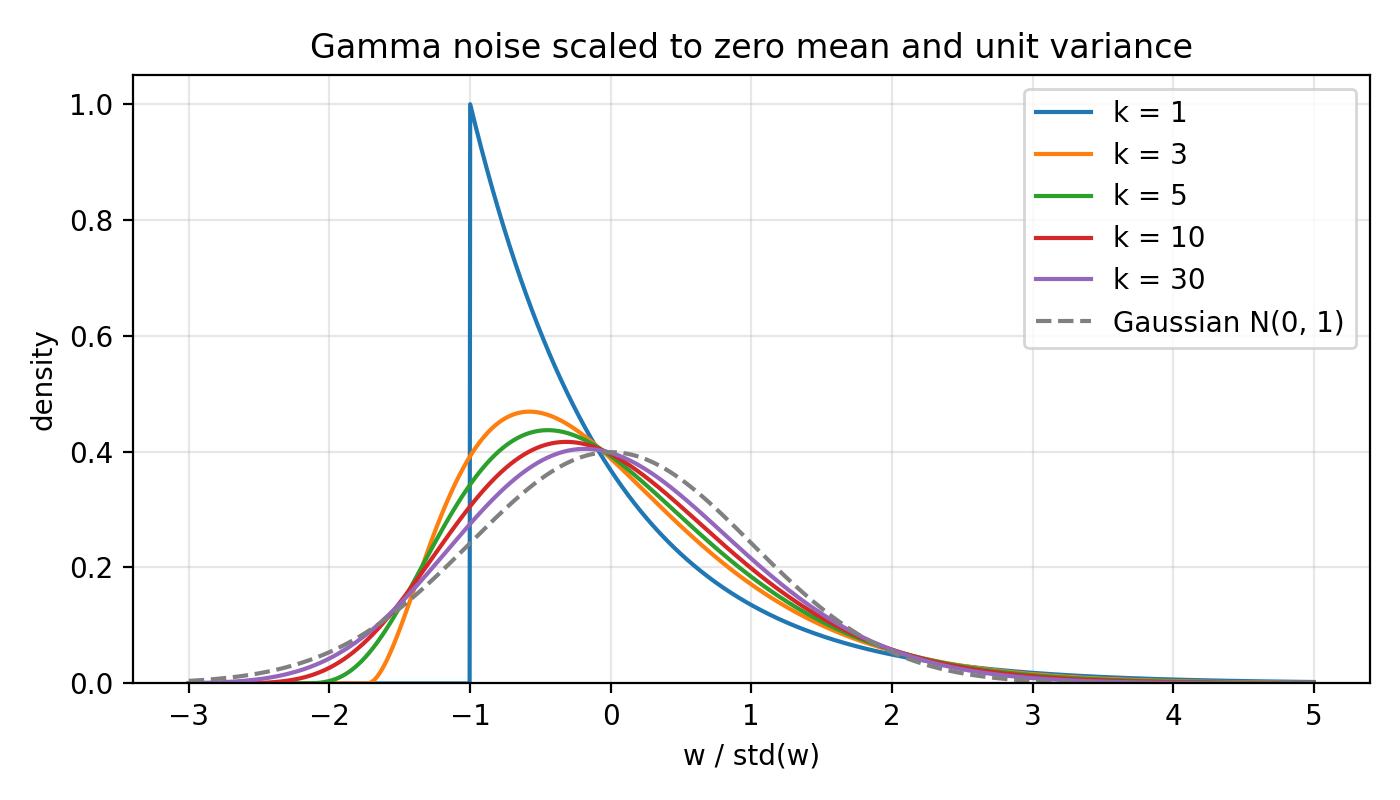
\includegraphics[width=\linewidth]{simD_gamma_density.png}
    \column{0.43\textwidth}
    \small
    \textbf{Noise:} $w = Y - k\theta$, \; $Y \sim \text{Gamma}(k, \theta)$.
    \begin{itemize}
      \item Zero mean, skewness $2/\sqrt{k}$.
      \item $k = 1$: exponential. Large $k$: almost Gaussian.
    \end{itemize}
    \vspace{0.4em}
    \textbf{CRLB} (valid for $k > 2$):
    \[
      \text{CRLB}_\gamma = \frac{(k-2)\,\theta^2}{N}
    \]
    \textbf{Mean (MSE):}
    \[
      \frac{\operatorname{Var}(\bar x)}{\text{CRLB}_\gamma} = \frac{k}{k-2}
    \]
  \end{columns}
\end{frame}

\begin{frame}{Gamma noise: simulation results}
  \begin{columns}[c]
    \column{0.55\textwidth}
    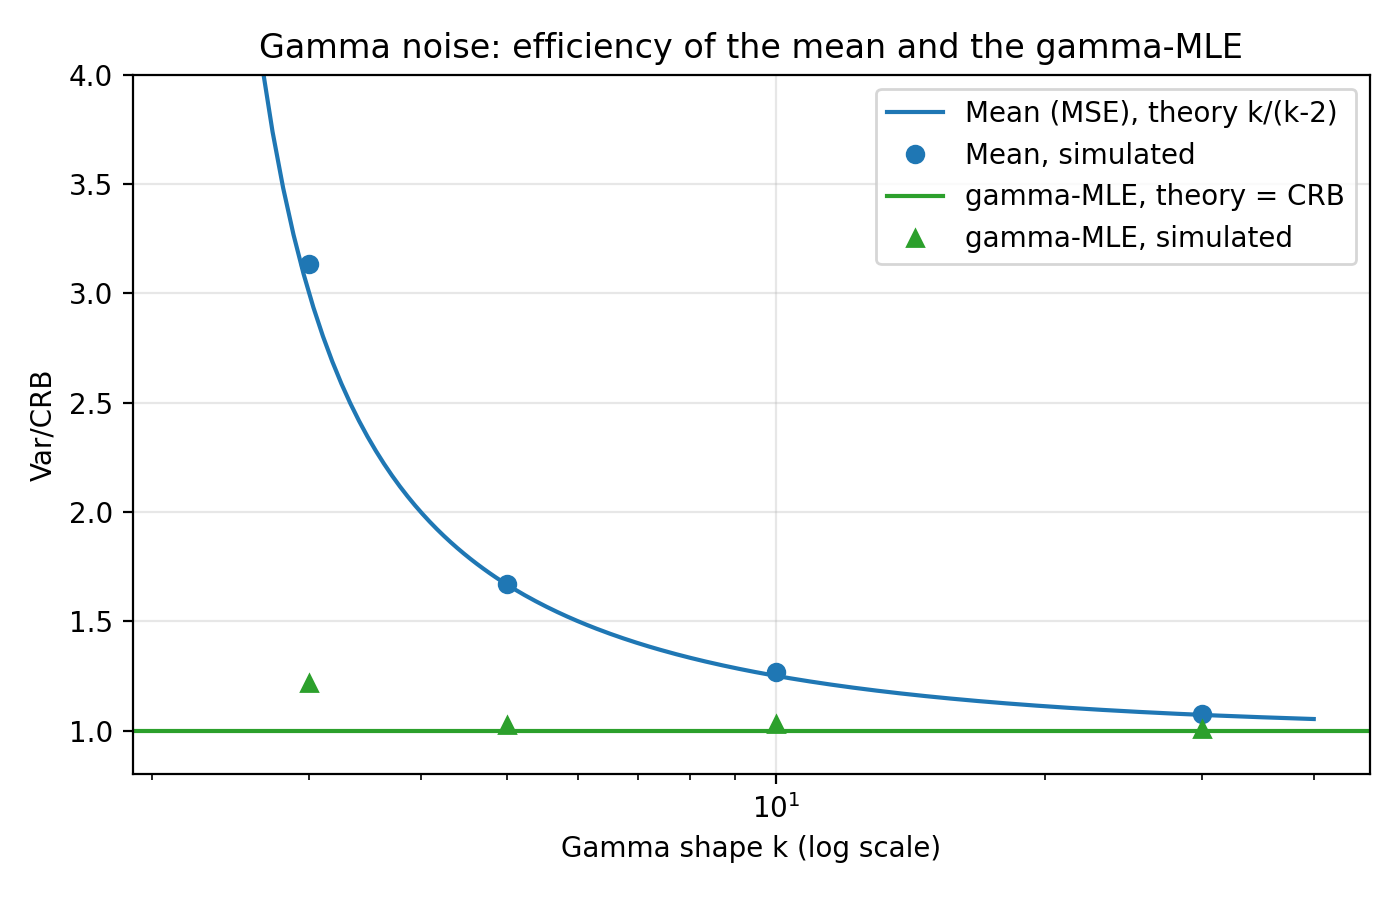
\includegraphics[width=\linewidth]{simD_gamma_ratio_vs_k.png}
    \column{0.43\textwidth}
    \small
    $A = 1$, $\theta = 1$, $N = 100$, 5000 trials.
    \begin{itemize}
      \item \textbf{Mean (MSE):} unbiased, but wastes data. $3\times$ the CRLB at $k = 3$.
      \item \textbf{Gamma MLE:} approaches the CRLB slowly ($1.18$ at $N = 100$, $1.04$ at $N = 1000$).
      \item \textbf{Median (MAE):} lands at about $A - \theta/3 \approx 0.67$ (0.69 at $k = 1$), not $A = 1$, for every $k$. More data does not fix it.
    \end{itemize}
  \end{columns}
\end{frame}

\begin{frame}{Below $k = 2$: no CRLB, but the edge is informative}
  \small
  The data have a hard left edge at $A - k\theta$. \textbf{Edge estimator:} $\hat A_{\text{edge}} = \min_n x[n] + k\theta$ (this \emph{is} the gamma MLE for $k \le 1$).
  \[
    \text{MSE}(\hat A_{\text{edge}}) \approx \theta^2\,\Gamma\!\left(1 + \tfrac{2}{k}\right)\Gamma(k+1)^{2/k}\,N^{-2/k}
    \qquad \text{vs} \qquad
    \text{MSE}(\bar x) = \frac{k\theta^2}{N}
  \]
  \vspace{-0.6em}
  \begin{center}
    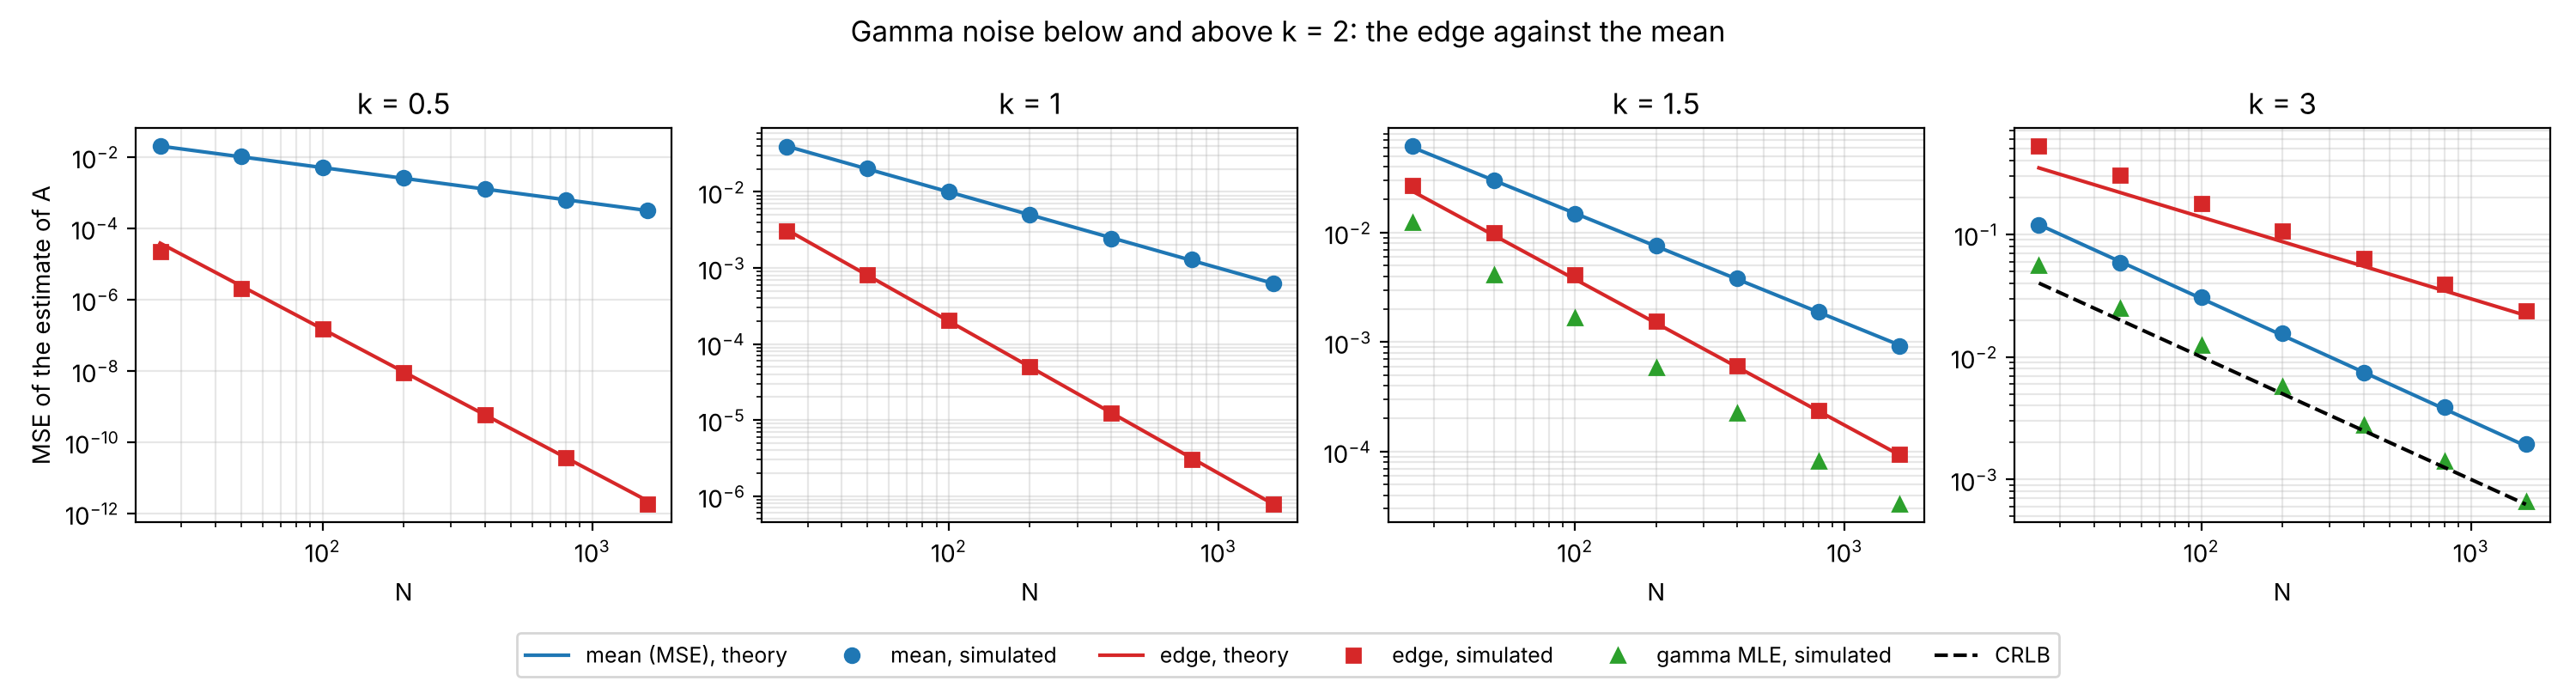
\includegraphics[width=0.92\linewidth]{simL_gamma_edge.png}
  \end{center}
  \vspace{-0.6em}
  \begin{itemize}
    \item $k < 2$: the edge wins, at rate $N^{-2/k}$. At $N = 100$, $k = 1$: \textbf{50$\times$} better than the mean.
    \item $k > 2$: the mean wins. $k = 2$ is exactly where the Fisher information becomes infinite.
  \end{itemize}
\end{frame}

% ============================================================
% PART 3 (next speaker): add your frames here
% ============================================================

% (Bhuvi's MCRB frames go here, before the Pareto part.)

% ---------- Harsh: Pareto noise (report Section 9), about 4 minutes ----------

\begin{frame}{When the bound breaks: Pareto noise}
  \begin{columns}[c]
    \column{0.55\textwidth}
    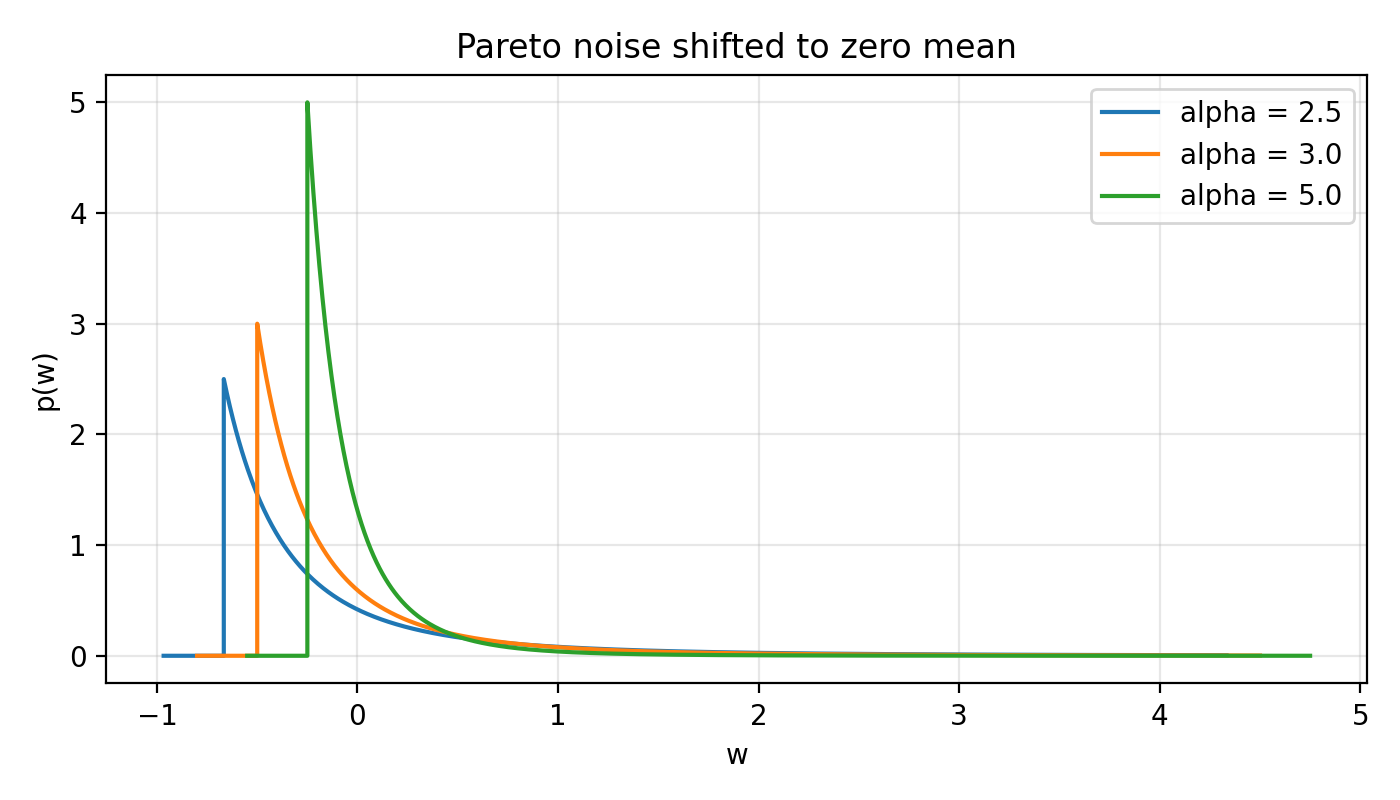
\includegraphics[width=\linewidth]{simF_pareto_density.png}
    \column{0.43\textwidth}
    \small
    $P \sim \text{Pareto}(\alpha)$: \; $p(p) = \dfrac{\alpha}{p^{\alpha+1}}$, \; $p \ge 1$.
    \vspace{0.3em}

    \textbf{Noise:} $w = P - \dfrac{\alpha}{\alpha - 1}$ (zero mean).
    \begin{itemize}
      \item Heavy power-law tail: $E[P^r]$ finite only for $r < \alpha$.
      \item \textbf{New feature:} the density does not start at zero. It \textbf{jumps} from $0$ to $\alpha$ at the left edge.
      \item The edge, $A - \frac{1}{\alpha-1}$, moves with $A$.
      \item Used for heavy-tailed radar sea clutter.
    \end{itemize}
  \end{columns}
\end{frame}

\begin{frame}{Why the CRLB does not apply}
  \small
  Score of one sample, with $u = $ the value of $P$:
  \[
    s(x; A) = \frac{\partial}{\partial A}\ln p(x; A) = \frac{\alpha + 1}{u},
    \qquad
    E[s] = (\alpha+1)\,E\!\left[\frac{1}{P}\right] = \alpha \;\neq\; 0 .
  \]
  \begin{itemize}
    \item The CRLB needs $E[s] = 0$. It fails here.
    \item Reason: the support moves with $A$. Differentiating $\int p(x;A)\,dx = 1$ gives an extra term equal to the \textbf{density at the edge}. It is zero only if the density is zero there. Here it is $\alpha$.
    \item Computing the formula anyway gives a \textbf{naive CRLB}:
    \[
      \text{naive CRLB} = \frac{\alpha + 2}{N\,\alpha(\alpha+1)^2} \qquad (\text{falls like } 1/N)
    \]
    \item We will see an estimator beat it by $100\times$, so it is not a valid bound.
  \end{itemize}
\end{frame}

\begin{frame}{Three estimators, and a bound that still holds}
  \small
  \begin{tabular}{lll}
    \toprule
    Estimator & Variance & Rate \\
    \midrule
    Mean (MSE) & $\dfrac{\alpha}{(\alpha-1)^2(\alpha-2)\,N}$ \; ($\alpha > 2$) & $1/N$ \\[1.2ex]
    Median (MAE) & $\approx \dfrac{2^{2/\alpha}}{N\alpha^2}$, biased: goes to $A + 2^{1/\alpha} - \frac{\alpha}{\alpha-1}$ & $1/N$ \\[1.2ex]
    Min-based & $\dfrac{N\alpha}{(N\alpha-1)^2(N\alpha-2)} \approx \dfrac{1}{(N\alpha)^2}$ & $\mathbf{1/N^2}$ \\
    \bottomrule
  \end{tabular}
  \vspace{0.5em}
  \begin{itemize}
    \item The minimum of $N$ Pareto($\alpha$) samples is Pareto($N\alpha$), so we can remove its bias exactly:
      $\hat A_{\min} = \min_n x[n] + \frac{\alpha}{\alpha-1} - \frac{N\alpha}{N\alpha - 1}$.
    \item \textbf{Chapman--Robbins bound} (no regularity needed): compare $A$ with a nearby $A + h$,
      \[
        \operatorname{Var}(\hat A) \ge \sup_{h > 0} \frac{h^2}{E_1(h)^N - 1}.
      \]
      If the data cannot tell $A$ from $A + h$, no estimator can be precise. As $h \to 0$ it becomes the CRLB when that is valid.
  \end{itemize}
\end{frame}

\begin{frame}{Pareto noise: simulation results}
  \begin{columns}[c]
    \column{0.55\textwidth}
    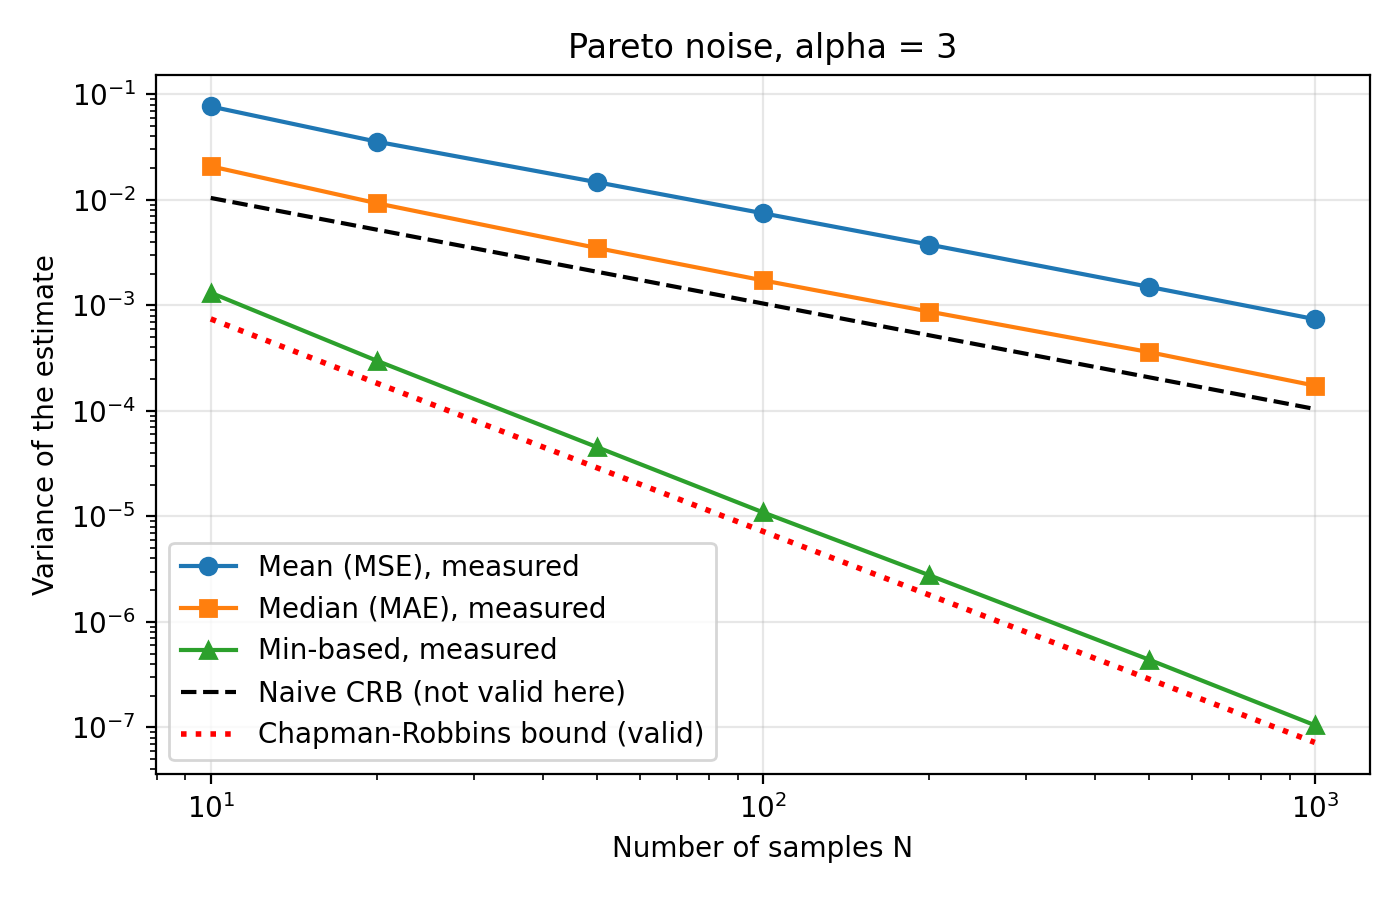
\includegraphics[width=\linewidth]{simF_pareto_var_vs_N.png}
    \column{0.43\textwidth}
    \small
    $A = 1$, $\alpha = 3$, 5000 trials.
    \begin{itemize}
      \item All measured variances match the formulas.
      \item At $N = 100$: min-based $1.16\times10^{-5}$ vs naive CRLB $1.04\times10^{-3}$: \textbf{almost $100\times$ below} the ``bound''.
      \item Slopes: mean, median, naive CRLB $-1$; min-based $-2.04$.
      \item Chapman--Robbins: slope $-2.01$, just below the min-based estimator. \textbf{Valid and nearly tight.}
    \end{itemize}
    \vspace{0.3em}
    \textbf{Takeaway:} a hard edge is very informative. MSE and MAE ignore it, so both are far from the best estimator.
  \end{columns}
\end{frame}

% ============================================================
% PART 4 (next speaker): add your frames here
% ============================================================

% ---------- Anshitha: real data (report Section 10), about 2 minutes ----------
% Placed after the MCRB part, because the standard-error result uses the MCRB.

\begin{frame}{Real data: French motor insurance claims}
  \begin{columns}[c]
    \column{0.55\textwidth}
    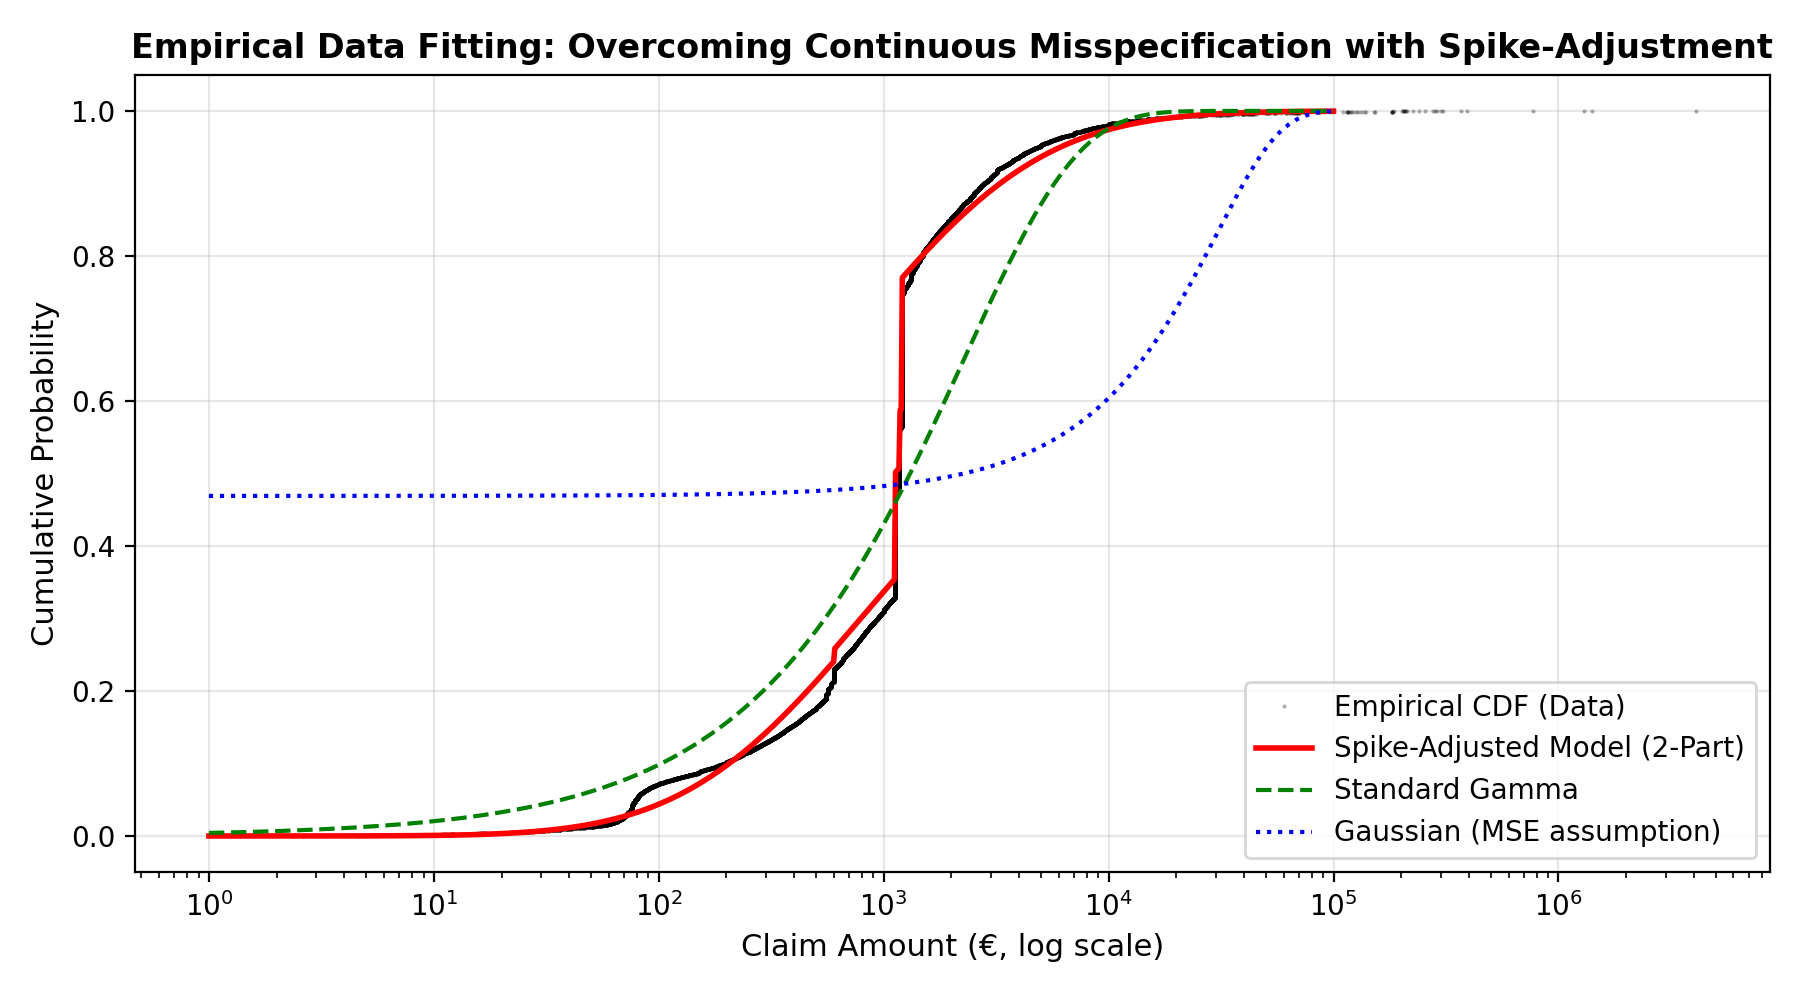
\includegraphics[width=\linewidth]{simI_spike_adjusted_cdf.png}
    \column{0.43\textwidth}
    \small
    26,639 claim amounts (\texttt{freMTPL2sev}). Noise unknown: we fit it.
    \begin{itemize}
      \item Mean $2279$, median $1172$.
      \item $42\%$ of claims sit on 5 fixed amounts. A two-part model (spikes + lognormal) fits them.
      \item Best gamma fit: $k = 0.69 < 1$. No CRLB exists.
      \item MSE vs MAE is a choice of \emph{what} to estimate, not of efficiency.
    \end{itemize}
  \end{columns}
\end{frame}

\begin{frame}{Real data: how precise is the mean?}
  \small
  \textbf{SE of the mean:} gamma model $16.8$ \;vs\; sample MCRB $179.5$ \;$\approx$\; bootstrap $177.0$
  \;$\Rightarrow$\; the wrong model is \textbf{$10.7\times$ overconfident}.
  \begin{center}
    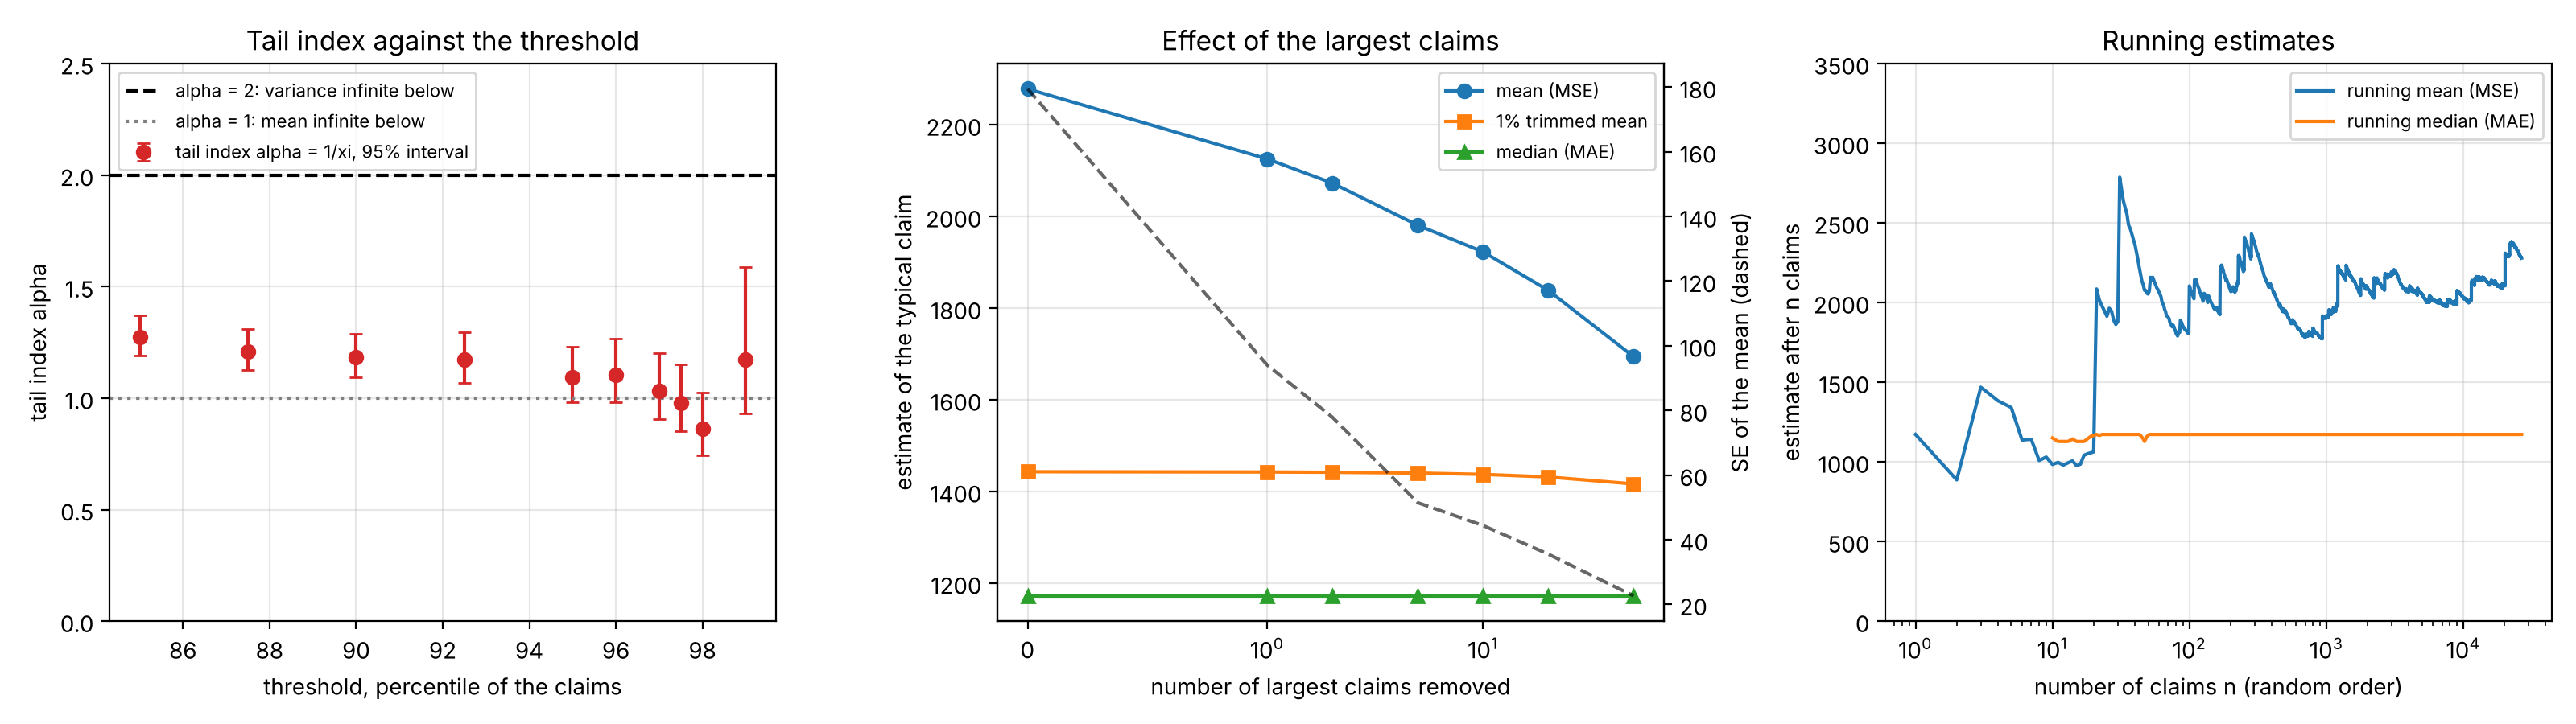
\includegraphics[width=\linewidth]{simM_claims_tail.png}
  \end{center}
  \vspace{-0.6em}
  \begin{itemize}
    \item Tail index $\alpha$ between $0.86$ and $1.28$ for every threshold: $\alpha < 2$, so the variance is \textbf{infinite}.
    \item Remove 1 claim of 26,639: the mean moves by 153 and its SE halves. The median never moves.
    \item \textbf{Takeaway:} on these data MAE gives a stable answer. MSE does not, and no error bar on it can be trusted.
  \end{itemize}
\end{frame}

% ---------- Harsh: neural networks (report Section 11), about 4 minutes ----------

\begin{frame}{Neural networks: the loss is still a noise model}
  \small
  From one number $A$ to a whole function:
  \[
    y = f^*(x) + w, \qquad f^*(x) = \sin(2\pi x) + 0.5x, \qquad x \sim \mathcal{U}[0, 1].
  \]
  \begin{itemize}
    \item Network $f_\theta$: MLP, 3 hidden layers of width 64, GELU, AdamW, 400 epochs. $N = 250$, 25 independent trials.
    \item Losses compared: MSE (Gaussian), MAE (Laplace), Huber, the matched likelihood, and \textbf{RCOS}, which picks the loss from the data.
    \item Noise: Gaussian ($\sigma = 0.3$), centered gamma ($k = 3$, skewed), Student-$t$ ($\nu = 3$, heavy tails).
  \end{itemize}
  \textbf{Error measure} over the 25 trained networks, with $\bar f$ their average:
  \[
    \text{Total risk} = \underbrace{\tfrac{1}{K}\textstyle\sum_k \big(\bar f(x_k) - f^*(x_k)\big)^2}_{\text{Bias}^2}
    + \underbrace{\tfrac{1}{K}\textstyle\sum_k \tfrac{1}{M}\sum_m \big(f^{(m)}(x_k) - \bar f(x_k)\big)^2}_{\text{Variance}}
  \]
  The same split as in the DC case: a wrong target shows up as bias, a wasteful loss as variance.
\end{frame}

\begin{frame}{RCOS: choosing the loss from the residuals}
  \small
  \begin{enumerate}
    \item Split the training data: $75\%$ to fit, $25\%$ to calibrate. The test set is never touched.
    \item Train a pilot network with Huber loss, and compute residuals $r_i$ on the calibration part.
    \item Measure skewness $\hat\gamma_1$, excess kurtosis $\hat\kappa$ and the tail ratio $\hat\sigma / \hat\sigma_{\text{MAD}}$.
    \item Choose the loss:
      \begin{itemize}
        \item $|\hat\gamma_1| \ge 0.45$ (skewed) $\Rightarrow$ gamma likelihood, with $\hat k = 4/\hat\gamma_1^2$
        \item $\hat\kappa \ge 0.8$ or tail ratio $\ge 1.22$ (heavy tails) $\Rightarrow$ Student-$t$ likelihood, $\hat\nu = \max(2.1,\, 4 + 6/\hat\kappa)$
        \item otherwise $\Rightarrow$ MSE
      \end{itemize}
    \item Retrain on all the training data with the chosen loss.
  \end{enumerate}
  \vspace{0.3em}
  The rules use the moment formulas of the earlier sections: gamma skewness $2/\sqrt{k}$, Student-$t$ excess kurtosis $6/(\nu - 4)$.
\end{frame}

\begin{frame}{Neural networks: simulation results}
  \small
  \begin{center}
  \begin{tabular}{lccc}
    \toprule
    Total risk (Bias$^2$) & Gaussian & Gamma ($k = 3$) & Student-$t$ ($\nu = 3$) \\
    \midrule
    MSE   & 0.068 (0.030) & 0.072 (0.033) & 0.079 (0.040) \\
    MAE   & 0.098 (0.056) & 0.096 (\textbf{0.052}) & 0.089 (0.047) \\
    Huber & 0.028 (0.009) & 0.047 (0.017) & 0.029 (0.007) \\
    RCOS  & 0.083 (0.039) & 0.082 (0.043) & \textbf{0.066} (0.022) \\
    \bottomrule
  \end{tabular}
  \end{center}
  $N = 250$, 25 trials.
  \begin{itemize}
    \item \textbf{Gaussian:} RCOS chose MSE in 25 of 25 trials, so it does not raise false alarms.
    \item \textbf{Student-$t$:} RCOS has $16\%$ less risk than MSE ($0.066$ vs $0.079$).
    \item \textbf{Gamma:} MAE has the largest bias ($0.052$ vs $0.033$ for MSE). It fits the conditional median, shifted from the mean as in the DC case.
    \item Huber, the pilot loss, has the lowest risk in all three regimes.
  \end{itemize}
\end{frame}

\begin{frame}{Neural networks on the insurance claims}
  \small
  Predict each claim from the policy features (driver age, vehicle, area, \dots). Test set: $20\%$ of the policies.
  \vspace{0.3em}
  \begin{columns}[c]
    \column{0.52\textwidth}
    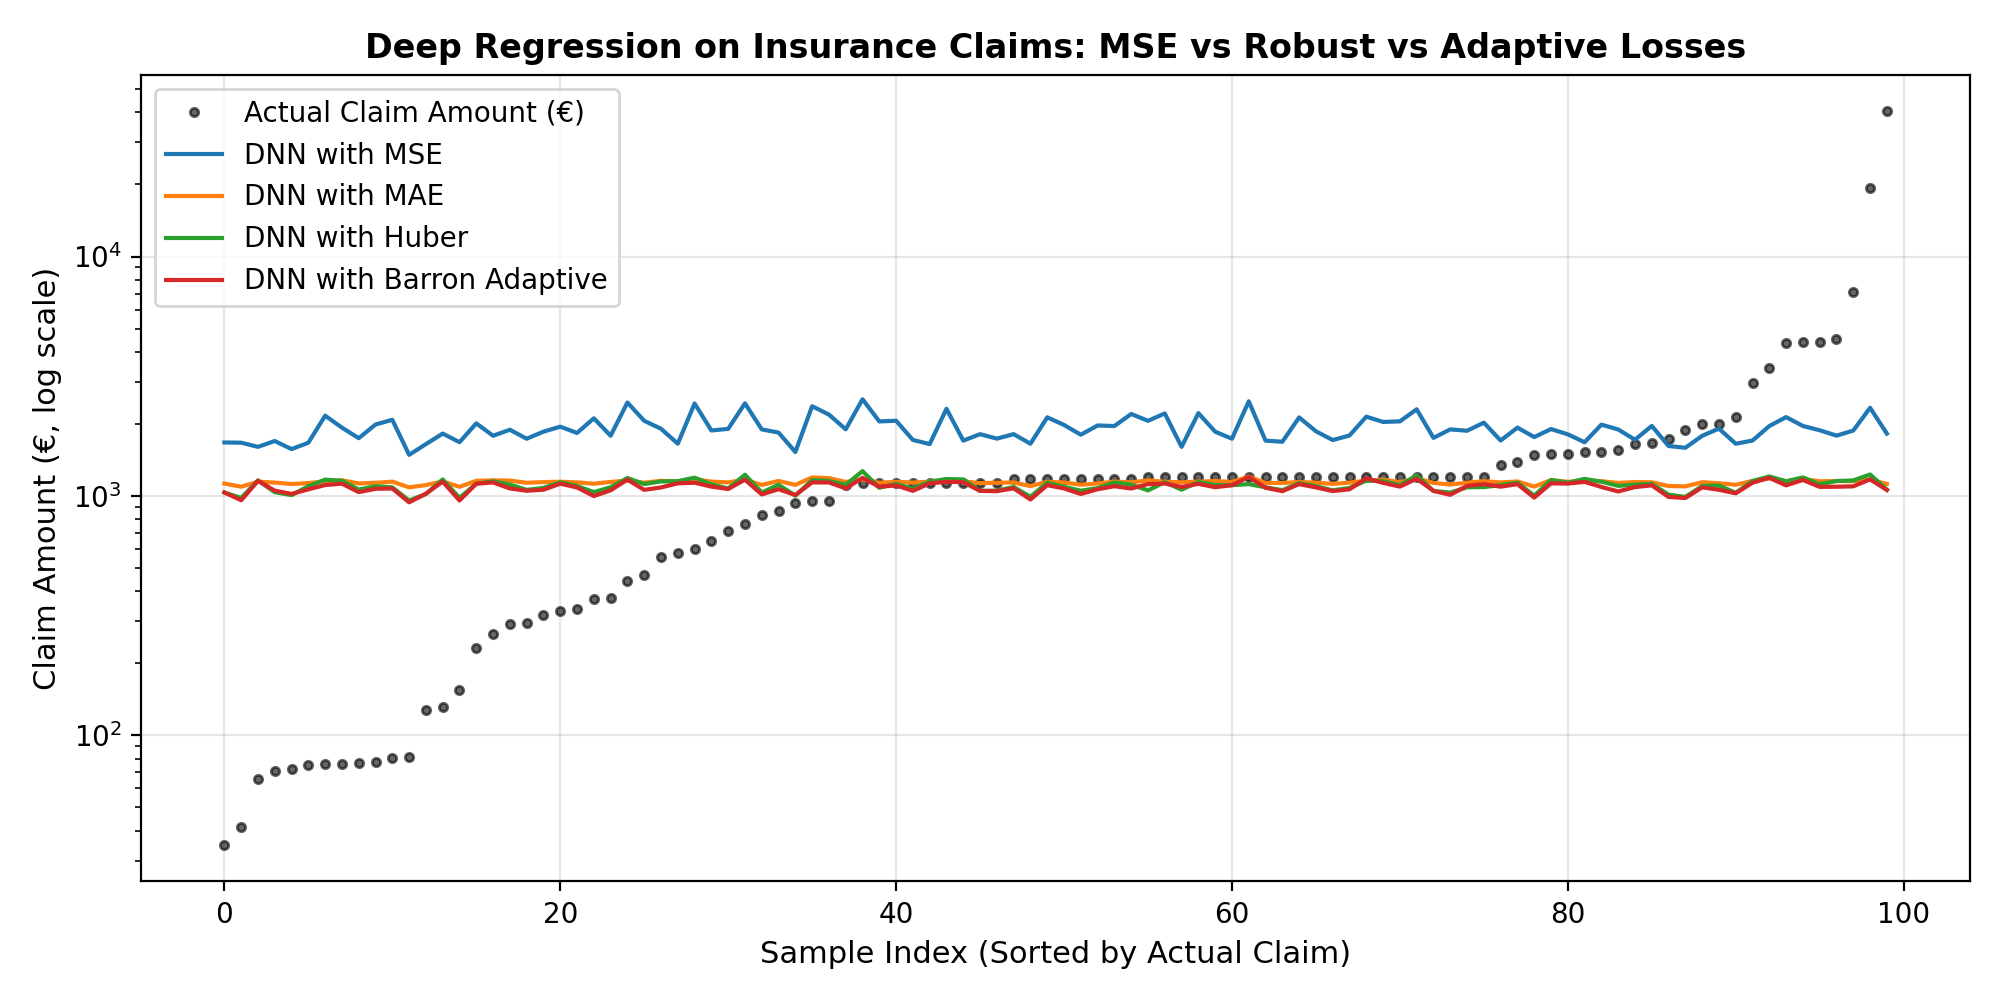
\includegraphics[width=\linewidth]{simNN_claims_predictions.png}
    \column{0.46\textwidth}
    \footnotesize
    \begin{tabular}{lcc}
      \toprule
      Loss & Typical error & Typical prediction \\
      \midrule
      MSE    & 876 & 1869 \\
      MAE    & 273 & 1143 \\
      Huber  & 269 & 1115 \\
      Barron & 268 & 1094 \\
      \bottomrule
    \end{tabular}

    (median absolute error and median prediction, euros)
    \begin{itemize}
      \item MSE predicts a typical claim of 1869, pulled up by the largest claims, with about $3\times$ the typical error.
      \item The robust losses stay near the 1172 median.
      \item Same lesson as the DC case: MSE estimates the mean, which the tail dominates.
    \end{itemize}
  \end{columns}
\end{frame}

% ---------- Anshitha: BACKUP slides. Remove the % signs to use them. ----------
%
% \begin{frame}{Backup: CRLB for gamma noise}
%   \small
%   Write $x = c + Y$ with left edge $c = A - k\theta$. Then
%   \[
%     \ln p(x; A) = (k-1)\ln(x - c) - \frac{x - c}{\theta} + \text{const},
%     \qquad
%     s = \frac{\partial \ln p}{\partial A} = -\frac{k-1}{Y} + \frac{1}{\theta}.
%   \]
%   Negative moments: $E[1/Y] = \dfrac{1}{\theta(k-1)}$, \; $E[1/Y^2] = \dfrac{1}{\theta^2(k-1)(k-2)}$.
%   \begin{itemize}
%     \item $E[s] = 0$ for $k > 1$ (regularity holds).
%     \item $i(A) = E[s^2] = \dfrac{1}{\theta^2(k-2)}$, finite only for $k > 2$.
%     \item The density goes to zero at the edge for $k > 1$, so the bound is valid even though the support moves with $A$.
%     \item $k \le 1$: density does not vanish at the edge, no CRLB (like Pareto).
%   \end{itemize}
% \end{frame}
%
% \begin{frame}{Backup: standard errors and removing the largest claims}
%   \small
%   \begin{center}
%   \begin{tabular}{lcccc}
%     \toprule
%     & Value & SE, gamma model & SE, sample MCRB & SE, bootstrap \\
%     \midrule
%     Mean (MSE)   & 2279 & 16.8 & 179.5 & 177.0 \\
%     Median (MAE) & 1172 & --   & --    & 0.0 \\
%     \bottomrule
%   \end{tabular}
%   \vspace{0.6em}
%   \begin{tabular}{rcccc}
%     \toprule
%     Removed & Mean & SE of mean & 1\% trimmed mean & Median \\
%     \midrule
%     0  & 2279 & 179.5 & 1443 & 1172 \\
%     1  & 2126 & 94.0  & 1442 & 1172 \\
%     5  & 1981 & 51.4  & 1440 & 1172 \\
%     50 & 1694 & 22.6  & 1416 & 1172 \\
%     \bottomrule
%   \end{tabular}
%   \end{center}
%   Median SE is 0 because the median sits on a fixed settlement amount (1172, 2072 claims).
% \end{frame}
%
% \begin{frame}{Backup: distribution fits to the claims}
%   \small
%   \begin{center}
%   \begin{tabular}{lcccc}
%     \toprule
%     Family & Parameters & Log-likelihood & AIC & KS \\
%     \midrule
%     Lognormal   & 2 & $-223590$ & $447184$ & 0.233 \\
%     Weibull     & 2 & $-227509$ & $455021$ & 0.204 \\
%     Gamma       & 2 & $-231154$ & $462312$ & 0.272 \\
%     Exponential & 1 & $-232593$ & $465188$ & 0.335 \\
%     Gaussian    & 2 & $-311788$ & $623579$ & 0.469 \\
%     \bottomrule
%   \end{tabular}
%   \end{center}
%   AIC $= 2p - 2\ln L$, lower is better. KS = largest gap between fitted and data CDF.
%   None fits well: the fixed-amount spikes and the very heavy tail.
% \end{frame}

\begin{frame}
  \centering
  \Large Thank you. Questions?
\end{frame}
\end{document}
